\documentclass[11pt]{article}

\usepackage{amsmath, amsthm}
\usepackage{setspace}
\usepackage{microtype, parskip, graphicx}
\usepackage[authoryear,sectionbib,sort]{natbib}
\usepackage{lineno}
\usepackage{longtable}
\usepackage{docmute}
\usepackage{caption, subcaption, multirow, morefloats, rotating}
\usepackage{wrapfig}
\usepackage{fullpage}
\usepackage{hyperref}

\frenchspacing
\doublespacing
\raggedright


\title{Species occurrence as a function of both emergent biological traits and environmental context}
\author{Peter D. Smits$^{1, \ast}$\\}
\date{}


\begin{document}

\maketitle

\noindent{}1. University of Chicago, Chicago, Illinois 60637.

\noindent{}$\ast$ Corresponding author; e-mail: psmits@uchicago.edu.

\bigskip

\textit{Manuscript elements}:

\bigskip

\textit{Keywords}:

\bigskip

\textit{Manuscript type}: Article

\bigskip

\noindent{\footnotesize Prepared using the suggested \LaTeX{} 
template for \textit{Am.\ Nat.}}

\linenumbers
\modulolinenumbers[2]

\newpage{}

%\begin{quotation}
  All the world's a stage, And all the men and women merely players; They have their exits and their entrances\dots
\end{quotation}
\attrib{Shakespeare, \textit{As You Like It}, Act II, Scene VII}

\begin{abstract}

  The set of species in a region changes over time as new species enter through speciation or immigration and as species leave the system through extinction and extirpation. How a regional species pool changes over time is the product of many processes acting at multiple levels of organization. Changes in the functional composition of a regional species pool are changes that occur across all local communities drawn from that species pool. While a speciess presence in a local community is due to the availability of the necessary biotic-biotic or biotic-abiotic interactions that enable coexistence, a species' presence in a regional species pool just requires that at least one local community has that set of necessary interactions. The goal of this analysis is to understand when, and possibly for what reasons, mammal ecotypes are enriched or depleted relative to their average diversity. Here, I analyze the diversity history of North American mammals ecotypes for most of the Cenozoic (the last 65 million years). This analysis frames mammal diversity in terms of both their means of interacting with the biotic and abiotic environment (i.e. functional group or ecotype) as well as their regional and global environmental context. Using two hierarchical Bayesian hidden Markov models of diversity, I find that changes to mammal diversity are driven more by the influx of new species than by selective extinction. I also find that the only ecotypes which experience a near constant increase in diversity over time are digitigrade and unguligrade herbivores, while arboreal ecotypes become increasingly rare and in many cases disappear entirely from the species pool over the Cenozoic. Additionally, I find that global temperature is only associated with the origination of some mammal ecotypes but, in almost all cases, does not affect the extinction of mammal ecotypes. %The clear and direct translation of research question to statistical model allows for precise and better contextualized results. By taking into account more of the complexity surrounding and contributing to species diversity and the diversification process, the idiosyncrasies of ecotype diversification histories are more clearly contextualized than before.


\end{abstract}


\documentclass[12pt,letterpaper]{article}

\usepackage{amsmath, amsthm}
\usepackage{microtype, parskip}
\usepackage[comma,numbers,sort&compress]{natbib}
\usepackage{lineno}
\usepackage{docmute}
\usepackage{caption, subcaption, multirow, morefloats, rotating}
\usepackage{wrapfig}
\usepackage{attrib}

\frenchspacing

\begin{document}

\section*{Introduction}
A regional species pool is the set of species which form communities in a specific region \citep{Mittelbach2015a} CITATIONS. Local scale processes like resource competition only affect the regional species pool if all communities are affected. The taxonomic and functional composition of a regional species pool changes over time due to speciation, migration, extinction. How do species pools change over time as species are recruited or go extinct? When are specific species ecologies enriched or depleted in the species pool? How does global and regional environmental context affect the set of species ecotypes (e.g. guilds) in a regional species pool? All of these questions fall under a single umbrella of analysis of ecotypic diversity and diversification.

% guilds and ecocube and ecotypes
Functional diversity is frequently broken into or thought of as a set of guilds, which are a set of species with similar sets of interactions and interactors (i.e. macroecology) \citep{Valentine1969,Bambach1977,Brown1989,Simberloff1991a,Wilson1999}. Species within a guild are expected to have more similar macroecological dynamics than species in different guilds. Building on the concept of guilds and a macroecological niche, \citet{Bush2007} presented a three-dimensional construct, or ecocube, for describing the macroecological role of a marine invertebrate species by their physical position (i.e. tiering), motility, and trophic role. Unique combinations along the three ecological trait axes indicate which among the possible ecotypes are observed. This approach has proven quite popular as it attempts to operationalize the guild concept in terms of shared characteristics that are indicative of the type of interactions experience by species of that macroecology \citep{Bush2007,Bambach2007,Bush2011,Bush2012b,Novack-Gottshall2007,Villeger2011}, but the overall utility of this approach is limited due to its condition as just a data type.

% how we think about mammal diversity
Previous analysis of mammal diversity and hypotheses as to the processes that have shaped it tend to be through one or more of the following lenses: diversity of an entire system (e.g. continent) \citep{Alroy2000g,Alroy1996a,Figueirido2012,Liow2008}, guild based \citep{Janis2004,Janis2000,Jernvall2004,Janis1993c,Pires2015a,Janis2008a}, clade based \citep{Quental2013,Slater2015c,Silvestro2015b,Fraser2015a,Cantalapiedra2017}, and environment based \citep{Blois2009,Janis1993c,Janis1993b,Fraser2015a,Eronen2015,Badgley2013,Badgley2017}. Rarely are more than two of these lenses considered simultaneously, and integration across the resulting diversity of observations and hypotheses tends to be based on coincidence. One of the goals of this study is to present a framework for simultaneously analyzing a diversity of hypotheses by integrating both species traits and environmental factors into a single model in order to infer a more holistic multi-level picture of the processes which may have shaped mammal species diversity and diversification.

% what we're dealing with in terms of hypotheses
The principle species trait considered in this study is a species' ecotype, defined here as the unique combination of species dietary cateogry and locomotor category (e.g. arboreal omnivore versus unguligrade herbivore). These classifications can be considered analogous to guilds or unique ecocube combinations as discussed above \citep{Bush2007,Bambach2007,Bush2011}. Species mass was also included as a species trait, but its inclusion is principally to control for that effect on the other covariates that are the focus of this study.

Translating previous work into hypotheses applicable to this analysis is difficult for a variety of reasons. Taxonomic groupings such as order or family are frequently invoked as an important factor in many proposed hypotheses for how mammal diversity is structured \citep{Quental2013,Slater2015c,Janis1993c,Pires2015a,Janis2008a}. Because taxonomic grouping conflates both species macroecology with shared evolutionary history, there are few clear ways to translate and operationalize these hypotheses in terms of macroecological change viewed through the lens of species interactions. Hypotheses as to macroecological change viewed through the lens of species interactions. Specifically, this issue arrises when trying to generalize previous observations from taxony-based framework to ecology-based one.

There is little convincing evidence of any major or sudden cross-ecotypic or cross-taxonomic turnover events in history of North American mammal diversity, unlike the Neogene record European mammals \citep{Alroy2009,Alroy1996a,Eronen2015,Janis1993b,Alroy2000g}. Instead of being concentrated in time, turnover has been found to be distributed through time. It is then expected then that, for this analysis, turnover events or periods of rapid diversification or depletion should not occur simultaneously for all ecotypes.

\citet{Jernvall2004} found that for the Neogene of Europe the relative abundance of mammal guilds was stable over time even in the face of high turnover rates, though they only considered large bodied taxa from a small set or mammal orders. Similar results have been observed for some taxonomic groups in North America \citep{Valkenburgh1999}. These results imply that there the types of interactions happening in local communities observed over a region are constant over time even if the interactors are constantly changing. \uppercase{more about diversity dependence here. what do people think the mammal diversity curve represents? can be anything if you think about it hard enough}.

The diversity history of ungulate herbivores has been characterized as more recently originating taxa having longer legs, higher crowned teeth, and a shift from graze-dominated to browse-dominated diets than their earlier originating counterparts \citep{Janis2004,Janis2000,Janis1993c,Janis2008a,Cantalapiedra2017,Fraser2015a}; all of which have all been attributed to some combination of environmental change itself or tectonic activity driving environmental change \citep{Janis2008a,Eronen2015,Blois2009,Badgley2017}. Additionally, it has been observed that these cursorial ungulate forms arose prior to cursorial carnivore forms, an observation attributed to the reorganization of plant communities towards the end of the Cenozoic and the latter emergence of ``modern'' environments and communities \citep{Janis1993c}.

Within the canid guild of North America (e.g. plantigrade and digitigrade carnivores) there is evidence that their diversity is self-regulating or somehow limited \citep{Valkenburgh1999}. Specifically, it has been proposed that different canid clades have replaced each other as the dominate members of that macroecological role within the species pool \citep{Silvestro2015b}. A pattern of generally constant diversity through time is also observed within the canid carnivore subguilds of hypercarnivore, hypocarnivore, and mesocarnivores identified by \citet{Slater2015c} even in the face of constant species turnover is consistent with limited possibility of increased diversity, even though there was no evidence of diversity-dependence in trait (e.g. body size) evolution \citep{Slater2015c}.

There is some uncertainty and a lack of consensus as to the effect of species body size on mammal diversity and aspects of the diversification processes, specifically extinction \citep{Liow2008,Liow2009,Tomiya2013,Smits2015b}. Species body size is frequently framed as an important biological descriptor because of how it is correlated with other important and relevant traits such as metabolic rate and home range size \citep{Brown1995}. It is also relatively easy to estimate for extinct species using proxy measures and regression equations, as was done in this study (see below). However, body size is normally considered without reference to other ecological descriptors of the species \citep{Liow2008}, but see \citep{Smits2015b}; this combined with the high amount of correlation between life history traits and body size limits processed-based inference because the actual causal mechanisms underlying an observed pattern are obscured or missing.

\citet{Smits2015b} found that the individual traits which form this study's ecotypes have strong effects on mammal extinction risk. Omnivorous taxa were found to have, on average, a greater duration than other dietary categories, while arboreal taxa were found to have a shorter duration than other locomotor categories \citep{Smits2015b}. Two possible scenarios that could yield this pattern were proposed: the extinction risk faced by arboreal is constant and high or the Paleogene and Neogene represent different regimes and extinction risk increased in the Neogene, thus driving up the Cenozoic average extinction risk. These two possible explanations have clear and testable predictions with respect to the diversity history of arboreal taxa: 1) the extinction risk arboreal taxa increased in the Neogene compared to the Paleogene, driving the average extinction risk of arboreal mammals up and leading to the loss of arboreal taxa from the species pool, or 2) if arboreal taxa have just a generally higher extinction risk than other ecotypes but have maintained a constant diversity for the Cenozoic. By inspecting the inferred diversity histories of the ecotypes, it should be possible to distinguish amoungst these hypotheses.

% if we control for one ecotype axis, what is variation along other axis?
% digitigrade vs unguligrade herbivores
% plantigrade vs digitigrade carnivores
% modernization of ecologies?
%   this is normally talked about in terms of taxonomic groups
%   how does this translate into ecologies?




% effect of climate on diversification process
Fundamentally, all species respond differently to climate and environmental change \citep{Blois2009}. Macroecological patterns are emergent patterns due to the similarities among species in how they respond to a similar ``stimulus.''

The effect of climate on diversity and the diversification process has been the focus of considerable research with a slight consensus favoring diversification being more biologically-mediated than climate-mediated \citep{Alroy1996a,Alroy2000g,Figueirido2012,Clyde1998a}. However, differences in temporal and geographic scale seem to underly the contrast between these two perspectives. For example when the mammal fossil record analyzed at small temporal and geographic scales a correlation between diversity and climate are observable \citep{Clyde1998a}. However, when the record is analyzed at the scale of the continent and most of the Cenozoic there is no correlation with diversity and climate \citep{Alroy2000g}. This results, however, does not go against the idea that there may be short periods of correlation and that the correlation between diversity and climate can change or even reverse direction over time; this type result means that there is no single direction of correlation between diversity and climate \citep{Figueirido2012}. 

In the case of a fluctuating correlation between diversity and climate it is hard to make the argument for an actual causal link between the two without modeling the underlying ecological differences between species; after all, species respond differently based on their individual ecologies \citep{Blois2009}. When analysis is based on diversity or taxonomy alone no mechanisms are possible to infer. Taxonomy, like body size, stands in for many important species traits to the point that mechanistic or process based inference is impossible. While emergent patterns might correspond to taxonomic grouping, this itself is an emergent phenomenon. Instead, by framing hypotheses in terms of species traits and their environmental context, these emergent phenomenon can be observed rather than assumed.

The climate history of the Cenozoic is generally characterized by a global cooling trend and the development of polar ice-caps during the Neogene; there are, of course, a few notable exceptions to this broad characterization \citep{Zachos2001,Zachos2008,Cramer2011}. The environmental context of North America for the Cenozoic is additionally characterized by an environmental transition from the closed, partially forested environments of the Paleogene to the savannah and grasslands environments of the Neogene \citep{Blois2009,Janis1993b,Janis2000,Stromberg2005}.

A lot of the climate and environmental changes observed for North America have been attributed to tectonic activity or uplift \citep{Blois2009,Eronen2015,Janis2008a,Badgley2013}. Tectonic uplift changes weather patterns (e.g. rain shadow) and mobilizes grit into the environment \citep{Jardine2012}. Increased grit in the environment combined with decreased rain fall is considered the primary reason behind the trend of increased hypsodonty, or high crowned teeth, among herbivore groups over the Cenozoic of both North America and Europe \citep{Jernvall2002,Jardine2012,Damuth2011}.

The Eocene-Oligocene transition has been observed to be associated with extinction of many ungulate taxa \citep{Janis2008a}. This boundary also marks the transition from the Paleogene to the Neogene and from herbivores being browsing dominated to grazing dominated, though not concurrently \citep{Janis1993b,Stromberg2005}. Additionally, the Paleogene-Neogene boundary marks the approximate start of Antarctic ice sheets, which were previously absent \citep{Zachos2008}. There is an observed stability in estimates of global temperature from the E/O transition till the end of the Miocene called the Mid-Miocene climatic optimum \citep{Zachos2001,Zachos2008}. The Mid-Miocene climatic optimum is bookended by periods of temperature decline. We would then expect that, for the Miocene, turnover and other diversification events would most likely be due to biological interactions or immigration and not biotic-abiotic interactions because of the constancy of the climate, and that those groups that are driven primarily by environmental factors, the Miocene would be a period of marked by an absence of major changes to diversity or the diversification process.

The environmental factors included in this study are estimates of global temperature and the changing floral groups present in North America across the Cenozoic CITATIONS. These covariates were chosen because they provide high level characterizations of the environmental context of the entire North American regional species pool for most of the Cenozoic. Importantly, the effects of a species ecotype on diversity are themselves modeled as functions of environmental factors (Fig. \ref{fig:concept_fourth_corner}) allowing for inference as to how a species ecology can mediate selective pressures do to its environmental context. 

\begin{figure}[ht]
  \centering
  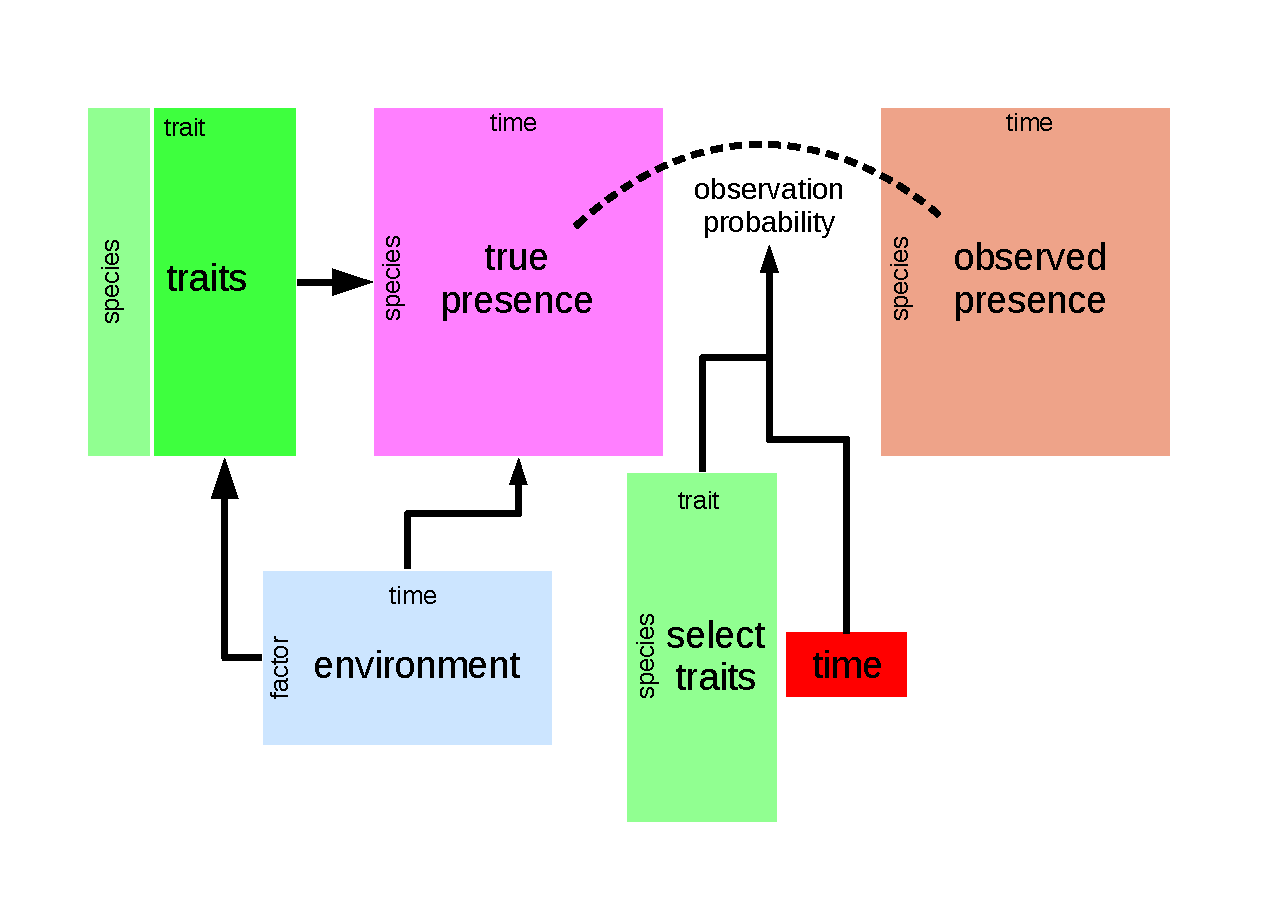
\includegraphics[width=\textwidth,height=0.5\textheight,keepaspectratio=true]{figure/paleo_fourth_corner}
  \caption[Conceptual diagram of the paleontological fourth-courner problem]{Conceptual diagram of the paleontological fourth corner problem. The observed presence matrix (orange) is the empirical presence/absence pattern for all species for all time points; this matrix is an incomplete observation of the ``true'' presence/absence pattern (purple). The estimated true presence matrix is modeled as a function of both environmental factors over time (blue) and multiple species traits (green). Additionally, the affect of environmental factors on species traits are also modeled as traits are expected to mediate the effects of a species environmental context. This diagram is based partially on material presented in \citet{Brown2014c} and \citet{Warton2015a}.}
  \label{fig:concept_fourth_corner}
\end{figure}

% 4th corner as similar but different lens
Fourth-corner modeling is an approach to explaining the patterns of either species abundance or presence/absence as a product of species traits, environmental factors, and the interaction between traits and environment \citep{Brown2014c,Warton2015a,Pollock2012,Jamil2013}; effectively uniting species distribution modeling (SDMs) with trait-based community assembly (CATS). In modern ecological studies, what is being modeled is species occurrences at localities distributed across a region \citep{Pollock2012,Jamil2013}. In this study, what is being modeled is the pattern of species occurrence over time for most of the Cenozoic in North America (Fig. \ref{fig:concept_fourth_corner}). By adding an additional dimension (time) to the fourth-corner framework we can gain better inference of how an instantaneous species pool (i.e. the Modern) is assembled over time. These two approaches, modern and palentologicial, are different views of the same three-dimensional pattern: species at localities over time. The temporal limitations of modern ecological studies and difficulties with uneven spatial occurrences of fossils in paleontological studies means that these approaches are complimentary but reveal different patterns of how species are distributed in time and space.

All observations, paleontological or modern, are made with uncertainty. With presence/absence data this uncertainty comes from now knowing if an absence is a ``true'' absence or just a failure to observe \citep{Royle2008,Royle2014,Foote1999a,Foote2001,Lloyd2011,Wang2016b}. For paleontological data, the incomplete preservation of whatever species were present into fossil form combined with incomplete sampling of what organisms were actually fossilized means that the true times of origination or extinction may not be observed \citep{Foote1999a,Foote2001,Wang2015,Wang2016b}.

Ultimately, the goals of this analysis are to understand when are unique ecotypes enriched or depleted in the North American mammal regional species pool and how changes in ecotypic diversity are related to changes in species' environmental context. In the analyses done here, many covariates which describe both a species' macroecology and its environmental context are considered. In order to analyze this complex and highly structured data set, I developed a hierarchal Bayesian model combing the forth-corner modeling approach with a model of an observation-occurrence or observation-origination-extinction process. The complexity and nuance inherent in questions that are focus of this study, it is possible to consider and test a large number of possible hypotheses. The hierarchical Bayesian modeling approach used here is appropriate for mitigating complications arising from both this complexity and the plethora of testable hypotheses (e.g. multiple comparisons, garden of forking paths) \citep{Gelman2013d,Gelman2012a,Gelman2014}.


\end{document}


\documentclass[12pt,letterpaper]{article}

\usepackage{amsmath, amsthm, amsfonts, amssymb}
\usepackage{microtype, parskip, graphicx}
\usepackage[comma,numbers,sort&compress]{natbib}
\usepackage{lineno}
\usepackage{longtable}
\usepackage{docmute}
\usepackage{caption, subcaption, multirow, morefloats, rotating}
\usepackage{wrapfig}
\usepackage{hyperref}

\frenchspacing

\begin{document}
\section*{Materials and Methods}

\subsection*{Taxon occurrences and species-level information}
All fossil occurrence information information was downloaded from the Paleobiology Database. Occurrences (PBDB) were restricted to all Mammalia sampled in North America between the Maastrichtian and Gelasian stages. Taxonomic, stratigraphic, and ecological metadata for each occurrence was included. The raw data is available for download at \url{http://goo.gl/2slgeU}.
%https://paleobiodb.org/data1.2/occs/list.csv?datainfo&rowcount&base_name=Mammalia&taxon_reso=species&interval=Maastrichtian,Gelasian&cc=NOA&show=class,genus,ecospace,loc,strat,stratext,lith,acconly. 

This raw data was then sorted, cleaned, and manipulated programmatically prior to analysis. Species taxonomic assignments given by the PBDB were updated for accuracy and consistency. For example, species classified in the order Artidodactyla were reclassified as Cetartiodactyla. These re-assignments follow \citet{Smits2015} and were based on CITATIONS. Additionally, Taxa who's life habit was classified as either volant (i.e. Chiroptera) or aquatic (e.g. Cetacea) were excluded from this analysis because of both differences in fossilization potential and applicability to the study of terrestrial species pools.

The life habit and dietary categories provided through the PBDB where coarsened to increase per ecotype sample size; this coarsening follows the same procedure as \citet{Smits2015}. Additionally, life habit category was further modified to break-up the vague ``ground-dwelling'' category; re-classifying these species by ankle posture gives more precise information about that species' environmental context. Ground-dwelling taxa were reassigned following \citet{Carrano1997} by species taxonomic context. Species ecotype is defined as the interaction between life habit and diet categories. Ecotype categories with less than 10 species havig ever been that combination were excluded, yielding a total of 18 of 21 possible ecotypes. % make a table.

\begin{table}[ht]
  \centering
  \caption{Species trait assignments in this study are a coarser version of the information available in the PBDB. Information was coarsened to improve per category sample size and uniformity and followed this table.}
  \begin{tabular}[ht]{ l | l | l }
    \hline
    \multicolumn{2}{ c |}{This study} & PBDB categories \\
    \hline \hline
    \multirow{4}{*}{Diet} & Carnivore & Carnivore \\
    & Herbivore & Browser, folivore, granivore, grazer, herbivore. \\
    & Insectivore & Insectivore. \\
    & Omnivore & Frugivore, omnivore. \\ 
    \hline
    \multirow{3}{*}{Locomotor} & Arboreal & Arboreal.\\
    & Ground dwelling & Fossorial, ground dwelling, semifossorial, saltatorial. \\
    & Scansorial & Scansorial. \\
    \hline
  \end{tabular}
  \label{tab:trait_cats}
\end{table}


\begin{center}
  \begin{longtable}{ l l l }
    \caption[Posture assignment based on taxonomy]{Posture assignment based on taxonomy} \label{tab:posture} \\

    Order & Family & Stance \\ \hline
    \endfirsthead
  
    \multicolumn{3}{p{\textwidth}}{{ \bfseries \tablename\ \thetable{} -- continued from previous page}} \\
    \hline Order & Family & Stance \\ \hline
    \endhead
      
    \hline \multicolumn{3}{p{\textwidth}}{{Continued on next page}} \\ \hline
    \endfoot
  
    \hline \hline
    \endlastfoot
  
    & Ailuridae & plantigrade \\ 
    & Allomyidae & plantigrade \\ 
    & Amphicyonidae & plantigrade \\ 
    & Amphilemuridae & plantigrade \\ 
    & Anthracotheriidae & digitigrade \\ 
    & Antilocapridae & unguligrade \\ 
    & Apheliscidae & plantigrade \\ 
    & Aplodontidae & plantigrade \\ 
    & Apternodontidae & scansorial \\ 
    & Arctocyonidae & unguligrade \\ 
    & Barbourofelidae & digitigrade \\ 
    & Barylambdidae & plantigrade \\ 
    & Bovidae & unguligrade \\ 
    & Camelidae & unguligrade \\ 
    & Canidae & digitigrade \\ 
    & Cervidae & unguligrade \\ 
    & Cimolodontidae & scansorial \\ 
    & Coryphodontidae & plantigrade \\ 
    & Cricetidae & plantigrade \\ 
    & Cylindrodontidae & plantigrade \\ 
    & Cyriacotheriidae & plantigrade \\ 
    & Dichobunidae & unguligrade \\ 
    Dinocerata &  & unguligrade \\ 
    & Dipodidae & digitigrade \\ 
    & Elephantidae & digitigrade \\ 
    & Entelodontidae & unguligrade \\ 
    & Eomyidae & plantigrade \\ 
    & Erethizontidae & plantigrade \\ 
    & Erinaceidae & plantigrade \\ 
    & Esthonychidae & plantigrade \\ 
    & Eutypomyidae & plantigrade \\ 
    & Felidae & digitigrade \\ 
    & Florentiamyidae & plantigrade \\ 
    & Gelocidae & unguligrade \\ 
    & Geolabididae & plantigrade \\ 
    & Glyptodontidae & plantigrade \\ 
    & Gomphotheriidae & unguligrade \\ 
    & Hapalodectidae & plantigrade \\ 
    & Heteromyidae & digitigrade \\ 
    & Hyaenidae & digitigrade \\ 
    & Hyaenodontidae & digitigrade \\ 
    & Hypertragulidae & unguligrade \\ 
    & Ischyromyidae & plantigrade \\ 
    & Jimomyidae & plantigrade \\ 
    Lagomorpha &  & digitigrade \\ 
    & Leptictidae & plantigrade \\ 
    & Leptochoeridae & unguligrade \\ 
    & Leptomerycidae & unguligrade \\ 
    & Mammutidae & unguligrade \\ 
    & Megalonychidae & plantigrade \\ 
    & Megatheriidae & plantigrade \\ 
    & Mephitidae & plantigrade \\ 
    & Merycoidodontidae & digitigrade \\ 
    Mesonychia &  & unguligrade \\ 
    & Mesonychidae & digitigrade \\ 
    & Micropternodontidae & plantigrade \\ 
    & Mixodectidae & plantigrade \\ 
    & Moschidae & unguligrade \\ 
    & Muridae & plantigrade \\ 
    & Mustelidae & plantigrade \\ 
    & Mylagaulidae & fossorial \\ 
    & Mylodontidae & plantigrade \\ 
    & Nimravidae & digitigrade \\ 
    & Nothrotheriidae & plantigrade \\ 
    Notoungulata &  & unguligrade \\ 
    & Oromerycidae & unguligrade \\ 
    & Oxyaenidae & digitigrade \\ 
    & Palaeomerycidae & unguligrade \\ 
    & Palaeoryctidae & plantigrade \\ 
    & Pampatheriidae & plantigrade \\ 
    & Pantolambdidae & plantigrade \\ 
    & Periptychidae & digitigrade \\ 
    Perissodactyla &  & unguligrade \\ 
    & Phenacodontidae & unguligrade \\ 
    Primates &  & plantigrade \\ 
    & Procyonidae & plantigrade \\ 
    & Proscalopidae & plantigrade \\ 
    & Protoceratidae & unguligrade \\ 
    & Reithroparamyidae & plantigrade \\ 
    & Sciuravidae & plantigrade \\ 
    & Sciuridae & plantigrade \\ 
    & Simimyidae & plantigrade \\ 
    & Soricidae & plantigrade \\ 
    & Suidae & digitigrade \\ 
    & Talpidae & fossorial \\ 
    & Tayassuidae & unguligrade \\ 
    & Tenrecidae & plantigrade \\ 
    & Titanoideidae & plantigrade \\ 
    & Ursidae & plantigrade \\ 
    & Viverravidae & plantigrade \\ 
    & Zapodidae & plantigrade \\ 
    \hline
  \end{longtable}
\end{center}



Species mass information was gathered from multiple different sources where a plurality of the body size estimates are from the PBDB. Body part measurements for many species are also available through the PBDB. Just as with \citet{Smits2015}, these measurements and corresponding regression equations were used to get mass estimates for more species. Additional mass estimates and body part measurements were sourced from CITATIONS, the Neogene Old World Database as in \citet{Smits2015}. Mass was log-transformed and then mean-centered and rescaled by dividing by two-times its standard deviation; this insures that the magnitude of effects for both continuous and discrete covariates are comparable and follows CITATION. % gelman and hill

\begin{table}[ht]
  \centering
  \caption{Regression equations used in this study for estimating body size. Equations are presented with reference to taxonomic grouping, part name, and reference.}
  \begin{tabular}{l | l | l | l}
    Group & Equation & log(Measurement) & Source \\
    \hline
    General & \(\log(m) = 1.827x + 1.81\) & lower m1 area &  \cite{Legendre1986} \\
    General & \(\log(m) = 2.9677x - 5.6712\) & mandible length & \cite{Foster2009a} \\
    General & \(\log(m) = 3.68x - 3.83\) & skull length & \cite{Luo2001} \\
    Carnivores & \(\log(m) = 2.97x + 1.681\) & lower m1 length & \cite{VanValkenburgh1990} \\
    Insectivores & \(\log(m) = 1.628x + 1.726\) & lower m1 area & \cite{Bloch1998} \\
    Insectivores & \(\log(m) = 1.714x + 0.886\) & upper M1 area & \cite{Bloch1998} \\
    Lagomorph & \(\log(m) = 2.671x - 2.671\) & lower toothrow area & \cite{Tomiya2013} \\
    Lagomorph & \(\log(m) = 4.468x - 3.002\) & lower m1 length & \cite{Tomiya2013} \\
    Marsupials & \(\log(m) = 3.284x + 1.83\) & upper M1 length & \cite{Gordon2003} \\
    Marsupials & \(\log(m) = 1.733x + 1.571\) & upper M1 area & \cite{Gordon2003} \\
    Rodentia & \(\log(m) = 1.767x + 2.172\) & lower m1 area & \cite{Legendre1986} \\
    Ungulates & \(\log(m) = 1.516x + 3.757\) & lower m1 area & \cite{Mendoza2006} \\
    Ungulates & \(\log(m) = 3.076x + 2.366\) & lower m2 length & \cite{Mendoza2006} \\
    Ungulates & \(\log(m) = 1.518x + 2.792\) & lower m2 area & \cite{Mendoza2006} \\
    Ungulates & \(\log(m) = 3.113x - 1.374\) & lower toothrow length & \cite{Mendoza2006} \\
    \hline
  \end{tabular}
  \label{tab:mass_est}
\end{table}


All fossil occurrences from 64 to 2 million years ago (Mya) were binned into 31 2 million year (My) bins. This temporal length was chosen because it is approximately the resolution of the North American mammal fossil record.



\subsection*{Environmental and temporal covariates}
The group-level covariates in this study are descriptors of species' environmental context, such as global temperature and floral interval. 

Global temperature was calculated from Mg/Ca isotope data across the Cenozoic CRAMER CITATION. \uppercase{why did i do this? tom ezard has used this and it is probably better than the zachos curve.} Two aspects of the Mg/Ca-based temperature curve were included in this analysis: mean and range. Both were calculated as the mean of all respective estimates for each 2 My temporal bins. Both mean and range were then rescaled as above: subtract mean, divide by twice the standard deviation.

Floral interval is a holistic descriptor of which taxonomic groups are present and their relative modernity of those taxa for a given temporal interval CITATION. Graham CITATION defines four intervals from the Cretaceous to the Pliocene; only three of these intervals are included in this analysis.


\subsection*{Modelling species occurrence}
Two different models were used in this study: a pure-presence model and a birth-death model. Both models at their core are hidden Markov model with an absorbing state. The difference between these two models is if the probability of a species origination and survival are considered equal or different. 

\subsubsection*{Data augmentation}
All presence/absence observations are incomplete. The hidden Markov model at the core of this analysis allows for observed absences to be used meaningfully to estimate the number of unobserved species. Of specific concern in this analysis is the unknown ``true'' size of the dataset; how many species could have actually been observed? While many species have been observed, the natural incompleteness of all observations, especially in the case of paleontological data, there are obviously many species which were never sampled.

Let \(N\) by the total number of observed species, \(M\) be the upper limit of possible species that could have existed given a model of species presence, and \(N^{\ast}\) is the all-zero histories where \(N^{\ast} = M - N\). This approach assumes that \(\hat{N} \sim \text{Binomial}(M, \psi)\) where \(\hat{N}\) is the estimated ``true'' number of species and \(\psi\) is the probability that any augmented species should actually be ``present.'' Because \(M\) is user defined, this approach effectively gives \(\psi\) a uniform prior over \(N\) to \(M\) CITATION. For a more detailed explanation of data augmentation and its application here, please see CITATION, CITATION, and CITATION. For this study, \(M = N + \lfloor{N / 4\rfloor}\).

Data imputation is the process of estimating missing data for partially observed covariates CITATION, this is simple in a Bayesian context because data are also parameters CITATION. Augmented species also have no known mass so a mass estimate must be imputed for each possible species CITATION ROYLE. This procedure assumes that mass values for augmented species are from the same distribution as observed species. The distribution of observed mass values is estimated as part of the model, and new mass values are then generated from this distribution. This approach is an example of imputing data missing completely at random CITATION. Because log mass values are rescaled as a part of this study, the body mass distribution is already known (\(\mathcal{N}(0, 0.5)\)); augmented species body mass just simply drawn from this distribution. 

In addition to body mass information, the augmented species need an ecotype classification. Because these species are completely unknown, they were all classified as ``augmented,'' an additional grouping indicating their unknown biology. This classification has no biological interpretation.



\subsubsection*{Observation process}
The type of hidden Markov model used in this study has three characteristic probabilities: probability \(p\) of observing a species given that it is present, probability \(\phi\) of a species surviving from one time to another, and probability \(\pi\) of a species first appearing CITATION. In this formulation, the probability of a species going extinct is \(1 - \pi\). For the pure-presence model \(\phi = \pi\), while for the birth-death model \(\phi \neq \pi\).

The probability of observing a species that is present \(p\) is modeled as a logistic regression was a time-varying intercept and species mass as a covariate. The effect of species mass on \(p\) was assumed linear and constant over time and given a prior reflecting a possible positive relationship; these assumptions are reflected in the structure of the model Equation \ref{eq:obs_model}. The parameters associated with this part of the model are described in Table \ref{tab:obs_param}.

\begin{table}
  \centering
  \caption{Observation parameters}
  \begin{tabular}{c l l}
    Parameter & dimensions & explanation \\
    \hline
    \(y\) & \(N \times T\) & observed species presence/absence \\
    \(z\) & \(N \times T\) & ``true'' species presence/absence \\
    \(p\) & \(T\) & probability of observing a species that is present at time \(t\) \\
    \(m\) & \(N\) & species log mass, rescaled \\
    \(\alpha_{0}\) & 1 & average log-odds of \(p\) \\ % when mass = 0
    \(\alpha_{1}\) & 1 & change in average log-odds of \(p\) per change mass \\
    \(r\) & \(T\) & difference from \(\alpha_{0}\) associated with time \(t\) \\
    \(\sigma\) & 1 & standard deviation of \(r\) \\
  \end{tabular}
  \label{tab:obs_param}
\end{table}

\begin{equation}
  \begin{aligned}
    y_{i, t} &\sim \text{Bernoulli}(p_{i, t} z_{i, t}) \\
    p_{i, t} &= \text{logit}^{-1}(\alpha_{0} + \alpha_{1} m_{i} + r_{t}) \\ 
    r_{t} &\sim \mathcal{N}(0, \sigma) \\
  \end{aligned}
  \label{eq:obs_model}
\end{equation}


\subsubsection*{Pure-presence process}
For the pure-presence model there is only a single probability dealing with the presence of a species \(\theta\). This probability was modeled as multi-level logistic regression with both species-level and group-level covariates CITATION. The parameters associated with pure-presence model are presented in Table \ref{tab:pres_param} and the full sampling statement in Equation \ref{eq:pure_presence}.

\begin{table}
  \centering
  \caption{Parameters for the model of presence in the pure-presence model}
  \begin{tabular}{c l l}
    Parameter & dimensions & explanation \\
    \hline
    \(z\) & \(N \times T\) & ``true'' species presence/absence \\
    \(\theta\) & \(N \times T - 1\) & probability of \(z = 1\) \\
    \(a\) & \(T - 1 \times D\) & ecotype-varying intercept; mean value of log-odds of \(\theta\) \\
    \(m\) & \(N\) & species log mass, rescaled \\
    \(b_{1}\) & 1 & effect of species mass on log-odds of \(\theta\) \\
    \(b_{2}\) & 1 & effect of species mass, squared, on log-odds of \(\theta\) \\
    \(U\) & \(T \times D\) & matrix of group-level covariates \\
    \(\gamma\) & \(U \times D\) & matrix of group-level regression coefficients \\
    \(\Sigma\) & \(D \times D\) & covariance matrix of \(a\) \\
    \(\Omega\) & \(D \times D\) & correlation matrix of \(a\) \\
    \(\tau\) & \(D\) & vector of standard deviations for each ecotype \(a_{d}\) \\
  \end{tabular}
  \label{tab:pres_param}
\end{table}

The species-level of the model (Eq. \ref{eq:pure_presence}) is a logistic regression with varying-intercept that varies by ecotype. Additionally, species mass was included as a covariate associated with two regression coefficients allowing a quadratic relationship with log-odds of occurrence. This assumption is based on the known distribution of mammal body masses where species with intermediate mass values are more common than either small or large bodied species. These assumptions are also reflected in the choice of priors for these regression coefficients.

The values of each ecotype's intercept are themselves modeled as regressions using the group-level covariates associated with environmental context. Each of these regressions has an associated variance of possible values of each ecotype's intercept CITATION. In addition, the covariances between ecotype intercepts, given this group-level regression, are modeled CITATION.

Following recommendations from CITATION, CITATION, CITATION all parameters not modeled elsewhere were given weakly informative priors. Weakly informative means that priors do not necessarily encode actual prior information but instead help regularize or weakly constrain posterior estimates. These priors have a concentrated probability density around and near zero; this has the effect of tempering our estimates and help prevent overfitting the model to the data CITATION. 

\begin{equation}
  \begin{split}
    y_{i, t} &\sim \text{Bernoulli}(p_{i, t} z_{i, t}) \\
    p_{i, t} &= \text{logit}^{-1}(\alpha_{0} + \alpha_{1} m_{i} + r_{t}) \\ 
    r_{t} &\sim \mathcal{N}(0, \sigma) \\
    z_{i, t} &\sim \text{Bernoulli}(\theta_{i, t}) \\
    \theta_{i, t} &= \text{logit}^{-1}(a_{t, j[i]} + b_{1} m_{i} + b_{2} m_{i}^{2}) \\
    a &\sim \text{MVN}(u \gamma, \Sigma) \\
    \Sigma &= \text{diag}(\tau) \Omega \text{diag}(\tau) \\
  \end{split}
  \begin{split}
    \alpha_{0} &\sim \mathcal{N}(0, 1) \\
    \alpha_{1} &\sim \mathcal{N}(1, 1) \\
    \sigma &\sim \mathcal{N}^{+}(1) \\
    b_{1} &\sim \mathcal{N}(0, 1) \\
    b_{2} &\sim \mathcal{N}(-1, 1) \\
    \gamma &\sim \mathcal{N}(0, 1) \\
    \tau &\sim \mathcal{N}^{+}(1) \\
    \Omega &\sim \text{LKJ}(2) \\
  \end{split}
  \label{eq:pure_presence}
\end{equation}


\subsubsection*{Birth-death process}
In the birth-death model, \(\phi \neq \pi\) and so each of these probabilities are modeled separately but in a similar manner to how \(\theta\) is modeled in the pure-presence model (Eq. \ref{eq:pure_presence}). The parameters associated with the birth-death presence model are presented in Table \ref{tab:bd_param} and the full sampling statement, including observation (Eq. \ref{eq:obs_model}), is described in Equation \ref{eq:birth_death}. 

\begin{table}
  \centering
  \caption{Parameters for the model of presence in the pure-presence model}
  \begin{tabular}{c l l}
    Parameter & dimensions & explanation \\
    \hline
    \(z\) & \(N \times T\) & ``true'' species presence/absence \\
    \(\phi\) & \(N \times T - 1\) & probability of \(z_{\textunderscore, t} = 1 | z_{\textunderscore, t - 1} = 0 \) \\
    \(\pi\) & \(N \times T - 1\) & probability of \(z_{\textunderscore, t} = 1 | z_{\textunderscore, t - 1} = 1 \) \\
    \(a^{\phi}\) & \(T - 1 \times D\) & ecotype-varying intercept; mean value of log-odds of \(\theta\) \\
    \(a^{\pi}\) & \(T - 1 \times D\) & ecotype-varying intercept; mean value of log-odds of \(\theta\) \\
    \(m\) & \(N\) & species log mass, rescaled \\
    \(b^{\phi}_{1}\) & 1 & effect of species mass on log-odds of \(\phi\) \\
    \(b^{\pi}_{1}\) & 1 & effect of species mass on log-odds of \(\pi\) \\
    \(b^{\phi}_{2}\) & 1 & effect of species mass, squared, on log-odds of \(\phi\) \\
    \(b^{\pi}_{2}\) & 1 & effect of species mass, squared, on log-odds of \(\pi\) \\
    \(U\) & \(T \times D\) & matrix of group-level covariates \\
    \(\gamma^{\phi}\) & \(U \times D\) & matrix of group-level regression coefficients \\
    \(\gamma^{\pi}\) & \(U \times D\) & matrix of group-level regression coefficients \\
    \(\Sigma^{\phi}\) & \(D \times D\) & covariance matrix of \(a^{\phi}\) \\
    \(\Sigma^{\pi}\) & \(D \times D\) & covariance matrix of \(a^{\pi}\) \\
    \(\Omega^{\phi}\) & \(D \times D\) & correlation matrix of \(a^{\phi}\) \\
    \(\Omega^{\pi}\) & \(D \times D\) & correlation matrix of \(a^{\pi}\) \\
    \(\tau^{\phi}\) & \(D\) & vector of standard deviations for each ecotype \(a^{\phi}_{d}\) \\
    \(\tau^{\pi}\) & \(D\) & vector of standard deviations for each ecotype \(a^{\pi}_{d}\) \\
  \end{tabular}
  \label{tab:bd_param}
\end{table}

Similar to the pure-presence model, both \(\phi\) and \(\pi\) are modeled as logistic regressions with varying-intercept and one covariate associated with two parameters. The possible relationships between mass and both \(\phi\) and \(\pi\) are reflected in the parameterization of the model and choice of priors (Eq. \ref{eq:birth_death}).

The intercepts of \(\phi\) and \(\pi\) both vary by species ecotype and those values are themselves the product of group-level regression using environmental factors as covariates (Eq. \ref{eq:birth_death}); this is identical to the pure presence model (Eq. \ref{eq:pure_presence}).

\begin{equation}
  \begin{split}
    y_{i, t} &\sim \text{Bernoulli}(p_{i, t} z_{i, t}) \\
    p_{i, t} &= \text{logit}^{-1}(\alpha_{0} + \alpha_{1} m_{i} + r_{t}) \\ 
    r_{t} &\sim \mathcal{N}(0, \sigma) \\
    \alpha_{0} &\sim \mathcal{N}(0, 1) \\
    \alpha_{1} &\sim \mathcal{N}(1, 1) \\
    \sigma &\sim \mathcal{N}^{+}(1) \\
    z_{i, 1} &\sim \text{Bernoulli}(\rho) \\
    z_{i, t} &\sim \text{Bernoulli}\left(z_{i, t - 1} \pi + \sum_{x = 1}^{t}(1 - z_{i, x}) \phi_{t}\right) \\
    \phi_{i, t} &= \text{logit}^{-1}(a^{\phi}_{t, j[i]} + b^{\phi}_{1} m_{i} + b^{\phi}_{2} m_{i}^{2}) \\
    \pi_{i, t} &= \text{logit}^{-1}(a^{\pi}_{t, j[i]} + b^{\pi}_{1} m_{i} + b^{\pi}_{2} m_{i}^{2}) \\
    a^{\phi} &\sim \text{MVN}(u \gamma^{\phi}, \Sigma^{\phi}) \\
    a^{\pi} &\sim \text{MVN}(u \gamma^{\pi}, \Sigma^{\pi}) \\
  \end{split}
  \begin{split}
    \Sigma^{\phi} &= \text{diag}(\tau^{\phi}) \Omega^{\phi} \text{diag}(\tau^{\phi}) \\
    \Sigma^{\pi} &= \text{diag}(\tau^{\pi}) \Omega^{\pi} \text{diag}(\tau^{\pi}) \\
    \rho &\sim \text{U}(0, 1) \\
    b^{\phi}_{1} &\sim \mathcal{N}(0, 1) \\
    b^{\pi}_{1} &\sim \mathcal{N}(0, 1) \\
    b^{\phi}_{2} &\sim \mathcal{N}(-1, 1) \\
    b^{\pi}_{2} &\sim \mathcal{N}(-1, 1) \\
    \gamma^{\phi} &\sim \mathcal{N}(0, 1) \\
    \gamma^{\pi} &\sim \mathcal{N}(0, 1) \\
    \tau^{\phi} &\sim \mathcal{N}^{+}(1) \\
    \tau^{\pi} &\sim \mathcal{N}^{+}(1) \\
    \Omega^{\phi} &\sim \text{LKJ}(2) \\
    \Omega^{\pi} &\sim \text{LKJ}(2) \\
  \end{split}
  \label{eq:birth_death}
\end{equation}


\subsection*{Posterior inference and model adequacy}
Programs that implement joint posterior inference for the above models (Eqs. \ref{eq:pure_presence}, \ref{eq:birth_death}) were implemented in the probabilistic programming language Stan CITATION. The models used here both feature latent discrete parameters in the large matrix \(z\) (Tables \ref{tab:obs_param}, \ref{tab:pres_param}, \ref{tab:bd_param}; Eqs. \ref{eq:obs_model}, \ref{eq:pure_presence}, \ref{eq:birth_death}). All methods for posterior inference implemented in Stan are derivative based which causes complications for actually implementing the above models because integers do not have derivatives. Instead of implementing a latent discrete parameterization, the posterior probabilities of all possible states of the latent parameters \(z\) were estimated (i.e. marginalized). 

Species durations at minimum range-through from the FAD to the LAD, but the incompleteness of all observations means that the actual time of origination or extinction is unknown. The marginalization approach used here means that the probabilities all possible histories for a species are calculated, from the end members of the species having existed for the entire study interval and the species having only existed between the directly observed FAD and LAD to all possible intermediaries CITATION. % this probably needs a figure to explain.

\begin{figure}[ht]
  \centering
  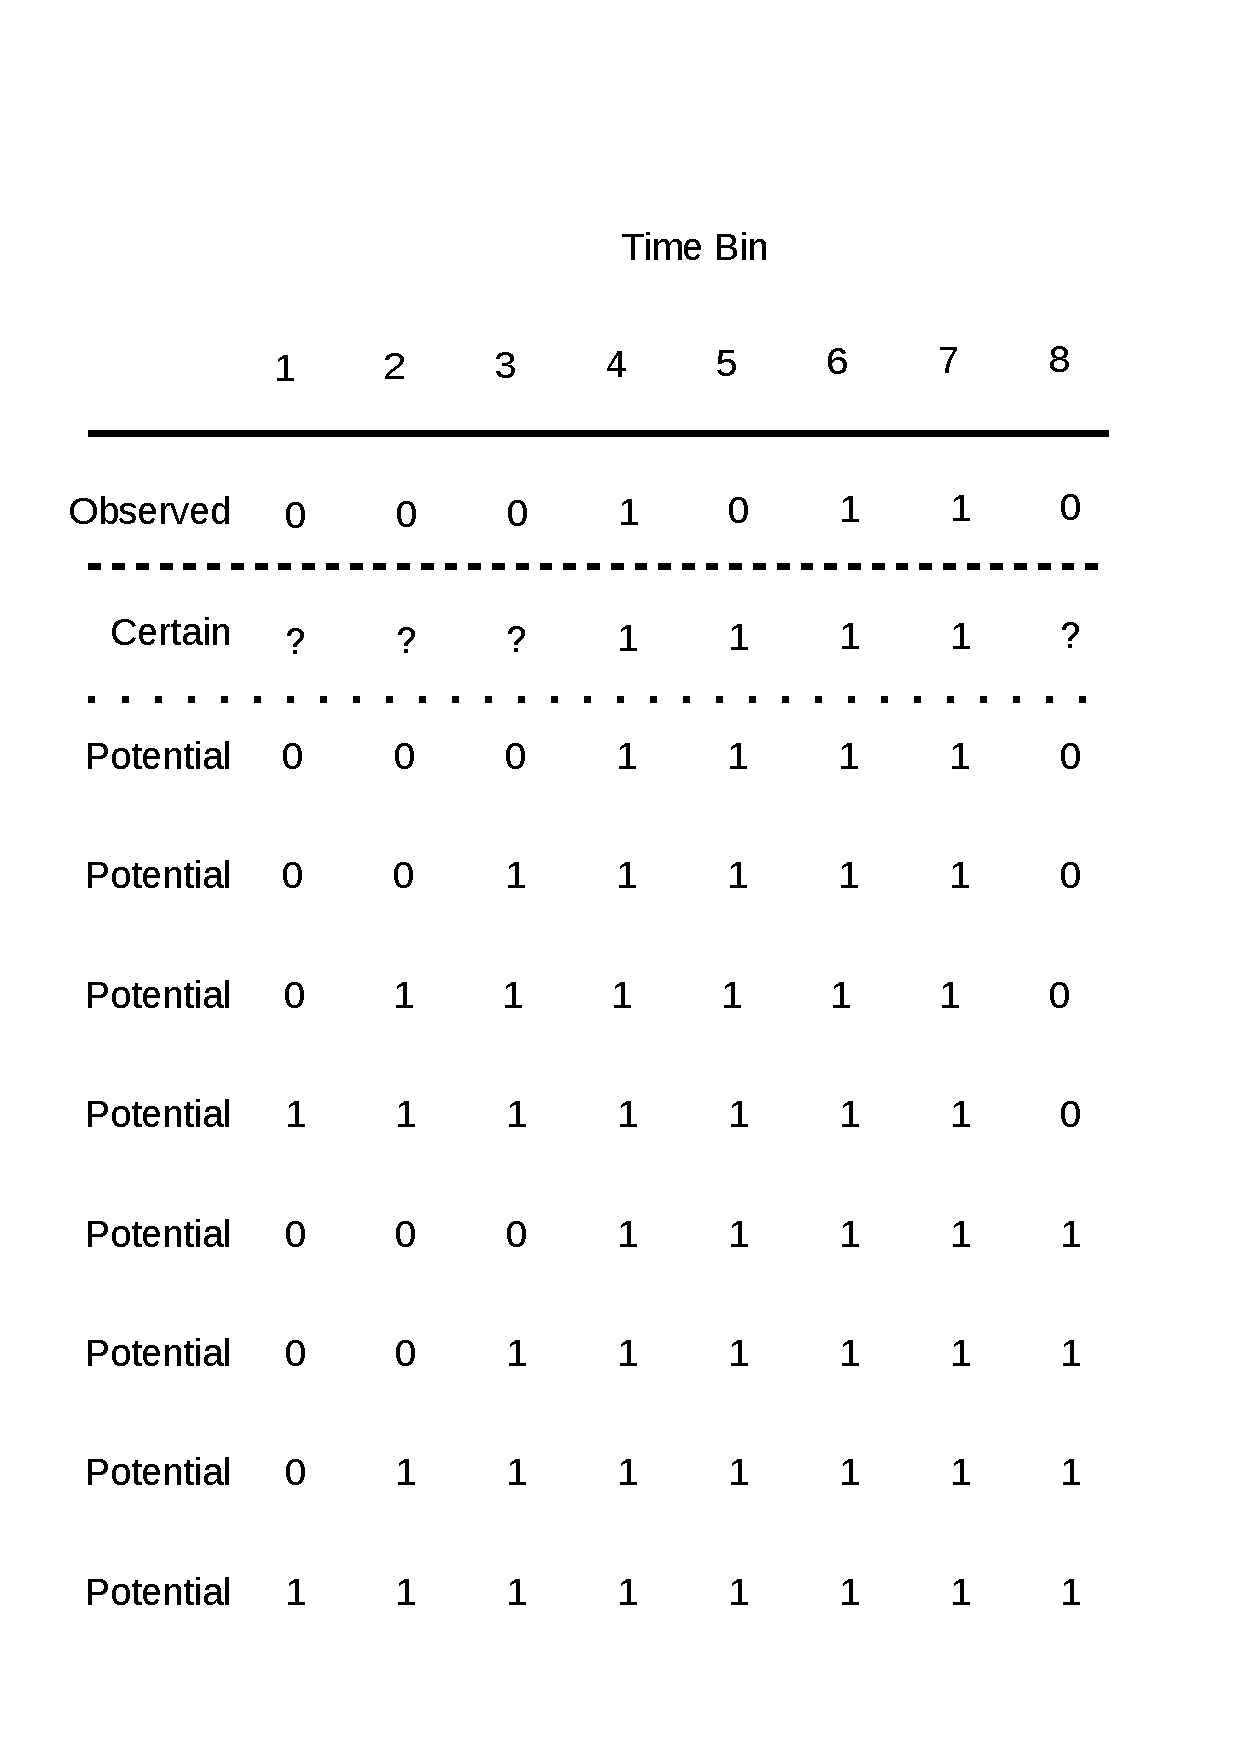
\includegraphics[height=0.5\textheight, width=\textwidth, keepaspectratio=true]{figure/margin}
  \caption[Conceptual figure of all possible occurrence histories for an observed species]{Conceptual figure of all possible occurrence histories for an observed species.}
  \label{fig:margin_concept}
\end{figure}


% Stan
%   version 2.9.0
%   marginalize over latent discrete parameters
%     keeping in mind that species HAVE to range through
%     sum of the log probability for all possible configutations
%     along with the sampling probability given those combinations as well
%     see code for implementation? 
%       it is kind of an annoying amount of math to write up

The combined size of the dataset and large number of parameters in both models (Eqs. \ref{eq:pure_presence}, \ref{eq:birth_death}), specifically the total number of latent parameters that are the matrix \(z\), means that stochastic approximate posterior inference is computationally very slow even using HMC. Instead, an approximate Bayesian approach was used: variational inference. A recently developed automatic variational inference algorithm called ``automatic differention variational inference'' (ADVI) is implemented in Stan and was used here CITATION. ADVI assumes that the posterior is Gaussian but still yields a true Bayesian posterior; this assumption is similar to quadratic approximation of the likelihood function used in maximum likelihood inference CITATION. The principal limitation of assuming the joint posterior is Gaussian is that the true topology of the log-posterior isn't represented; this is a particular burden for scale parameters which are bound to be positive (e.g. standard deviation).

After fitting both models (Eqs. \ref{eq:pure_presence}, \ref{eq:birth_death}) using ADVI, model adequacy and quality of fit was assessed using a series of posterior predictive checks CITATION CITATION. Because all Bayesian models are inherently generative, simulations of new data sets is ``free'' CITATION. By simulating many theoretical data sets using the observed covariate information the congruence between predictions made by the model and the observed empirical data can be assessed. By combining multiple posterior predictive tests of congruence between empirical and simulated values of interest, the holistic adequacy of the model can be analyzed CITATION.

An example posterior predictive check used in this study was comparing the observed average number of observations per species to a distribution of simulated averages; if the empirically observed value sits in the middle of the distribution than the model is adequate in reproducing the observed number of occurrences per species. 

Posterior simulations for time series are start with the values at t = 1 and then just simulating forward. 



\end{document}


\documentclass[12pt,letterpaper]{article}

\usepackage{amsmath, amsthm}
\usepackage{microtype, parskip}
\usepackage[comma,numbers,sort&compress]{natbib}
\usepackage{lineno}
\usepackage{docmute}
\usepackage{caption, subcaption, multirow, morefloats, rotating}
\usepackage{wrapfig}

\frenchspacing

\begin{document}

\section*{Results}

Posterior results take one of two forms: direct inspection of parameter estimates, and downstream estimates of diversity and diversification rates. For the former, both the pure-presence and birth-death models (Eq. \ref{eq:pure_presence}, and \ref{eq:birth_death} are inspected. For the latter, only posterior estimates from the birth-death model are considered; the reason for this is explained below in the comparison of the models' posterior predictive check results.

\subsection*{Comparing parameter estimates from the pure-presence and birth-death models}

% look at the posterior predictive checks
%   which model has better fit
%   what does that mean?

Comparison of the posterior predictive performance of the pure-presence and birth-death models reveals a striking difference in quality of the models' fits to the data (Fig. \ref{fig:ppc_pure_presence} and \ref{fig:ppc_birth_death}). The birth-death model is clearly able to reproduce the observed average number of occurrence, in contrast to the pure-birth model which greatly underestimates the ovserved average number of occurrences. The interpretation of these results is that the results of the birth-death model are more representative of the data than the pure-presence model, though further inspection of the posterior parameter estimates can provide further insight into why these models give different posterior predictive results \citep{Gelman2013d}.

\begin{figure}[ht]
  \centering
  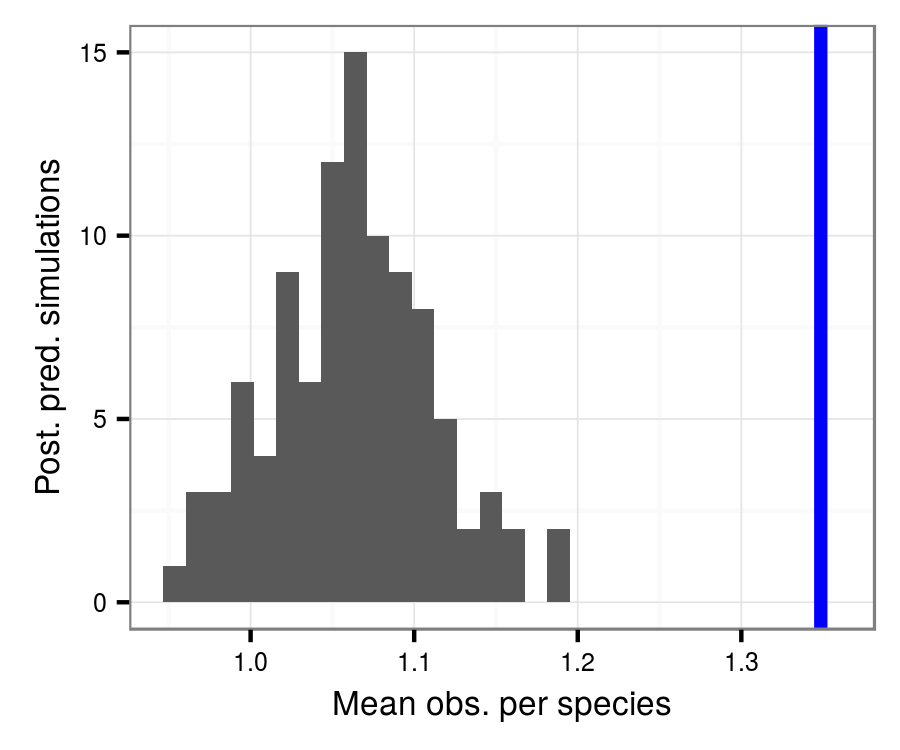
\includegraphics[width=\textwidth,height=0.4\textheight,keepaspectratio=true]{figure/pred_occ}
  \caption[Posterior predictive check for pure-presence model]{Comparison of the average observed number of occurrences per species (blue line) to the average number of occurrences from 100 posterior predictive datasets using the posterior estimates from the pure-presence model.}
  \label{fig:ppc_pure_presence}
\end{figure}

\begin{figure}[ht]
  \centering
  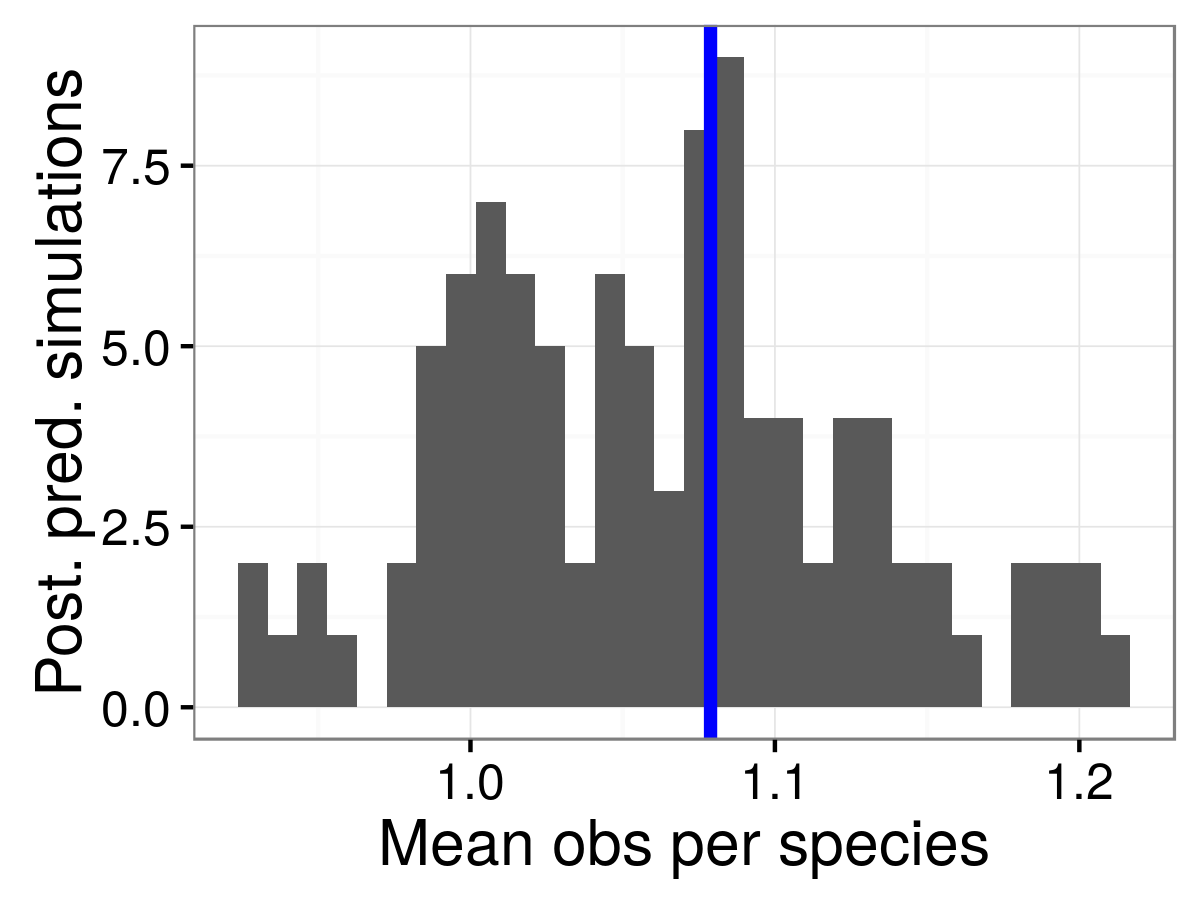
\includegraphics[width=\textwidth,height=0.4\textheight,keepaspectratio=true]{figure/pred_occ_bd}
  \caption[Posterior predictive check for birth-death model]{Comparison of the average observed number of occurrences per species (blue line) to the average number of occurrences from 100 posterior predictive datasets using the posterior estimate from the birth-death model.}
  \label{fig:ppc_birth_death}
\end{figure}


% need to inspect the posterior estimates in order to understand the differences
%   ecotype occurrence (pp), origination + survival (bd) probabilities
%   effect of mass on 
%     preservation (pp, bd)
%     occurrence (pp)
%     origination + survival (bd)
%   group-level covariates on 
%     occurrence (pp)
%     origination + survival (bd)

Occurrence probabilities estimated from the pure-presence model (Fig. \ref{fig:eco_occur}) are much more similar to the origination estimates from the birth-death model (Fig. \ref{fig:eco_origin}) than the estimates of survival probability (Fig. \ref{fig:eco_survival}). 

In general, both occurrence probabilities estimated from the pure-presence model (Fig. \ref{fig:eco_occur}) and origination probabilities estimated from the birth-death model (fig. \ref{fig:eco_origin}) increase with time. Notable, ecotypes with arboreal components do not follow this average; instead, occurrence and origination probabilities appear relatively flat for most of the Cenozoic.

The dramatic differences between origination and survival probabilities indicate how different these processes are, and may be responsible for the better posterior predictive perfomance of the birth-death model over the pure-presence model (Fig. \ref{fig:ppc_pure_presence}, and \ref{fig:ppc_birth_death}). While the estimates of both time series have high variance, what is striking is how mean origination probability changes over time while in general survival probabilities have relatively stable means (Fig. \ref{fig:eco_origin}, and \ref{fig:eco_survival}).

Estimates of origination probabilities appear to have less uncertainty than for survival (Fig. \ref{fig:eco_origin}, and \ref{fig:eco_survival}).


\begin{figure}[ht]
  \centering
  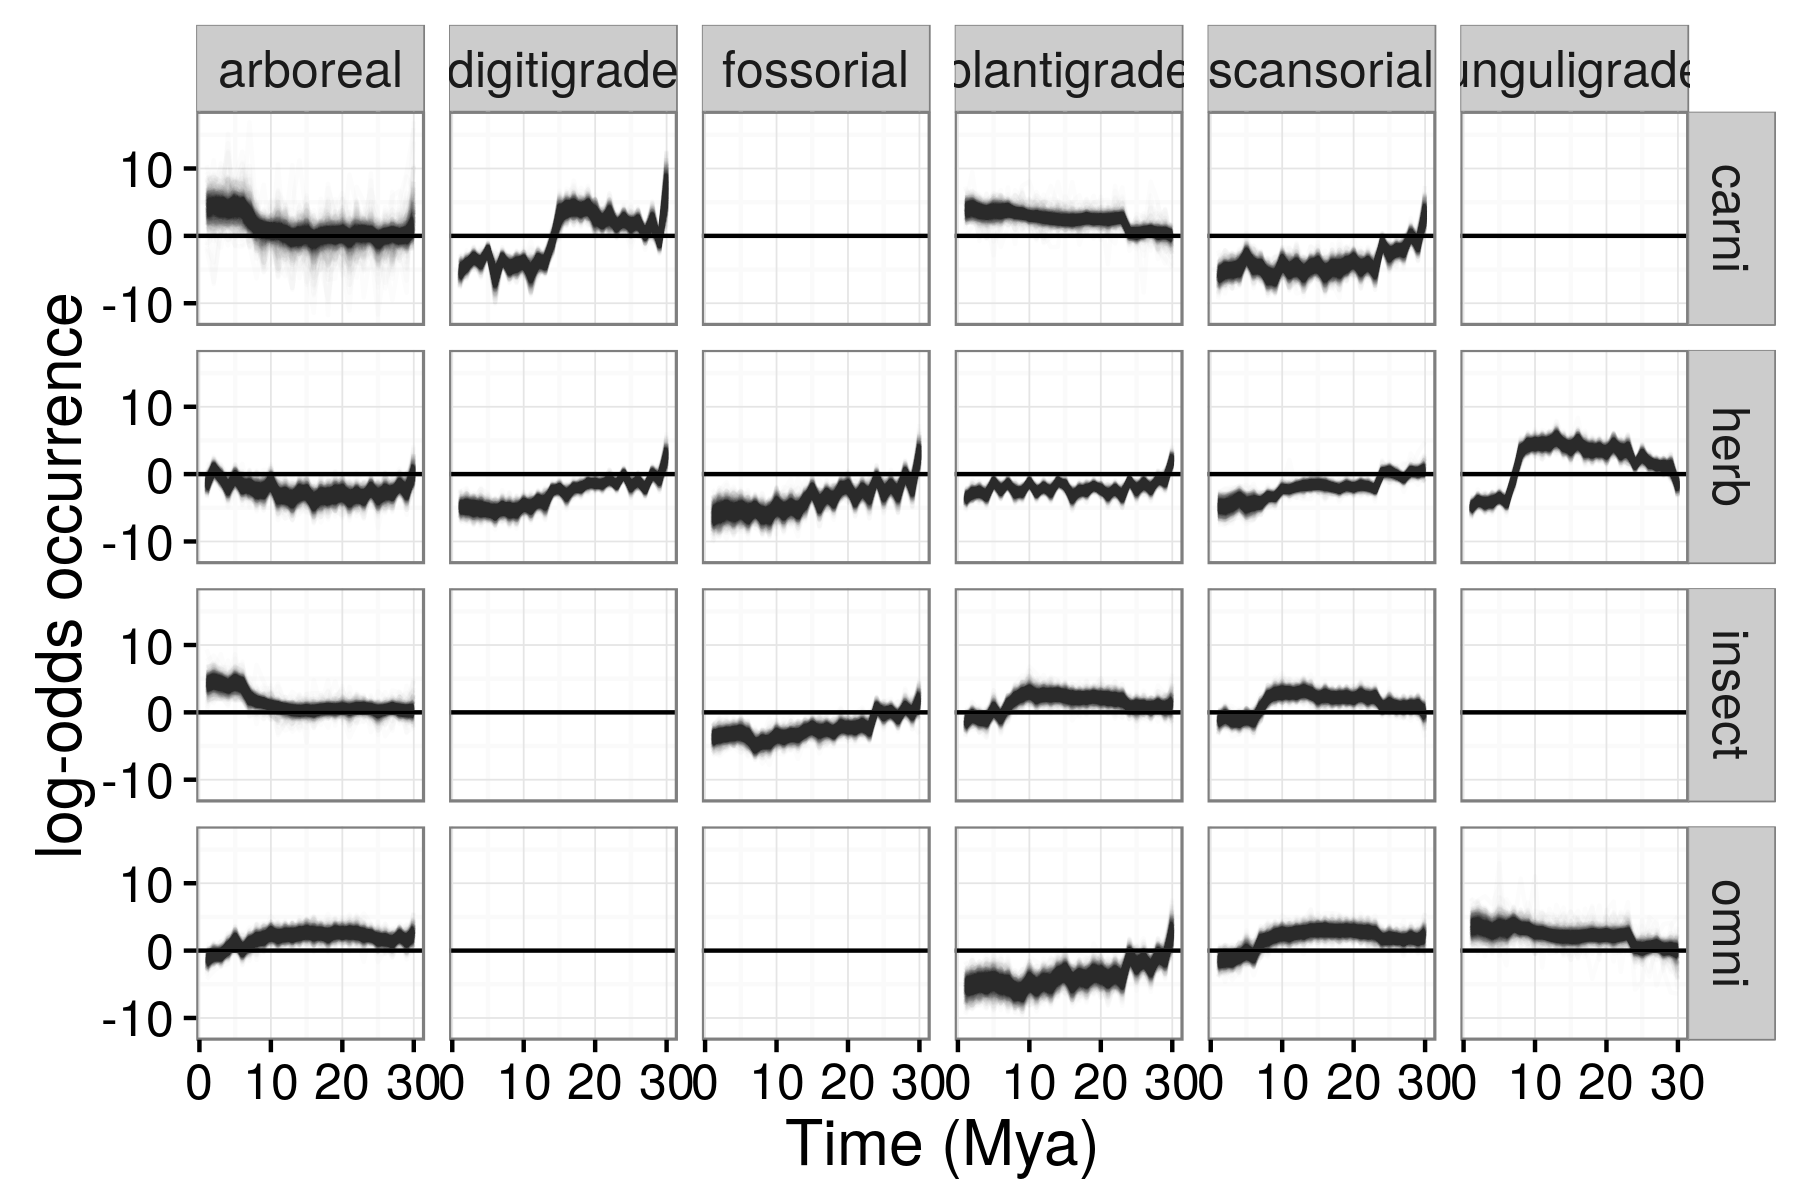
\includegraphics[width=\textwidth,height=0.8\textheight,keepaspectratio=true]{figure/ecotype_occurrence}
  \caption[Ecotype occurrence probability estimated from the pure-presence model]{Probability of a mammal ecotype occurring over time as estimated from the pure-presence model. Each panel depicts 100 random samples from the model's posterior. The columns are by locomotor category and rows by dietary category; their intersections are the observed and analyzed ecotypes. Panels with no lines are ecotypes not observed in the dataset.}
  \label{fig:eco_occur}
\end{figure}

\begin{figure}[ht]
  \centering
  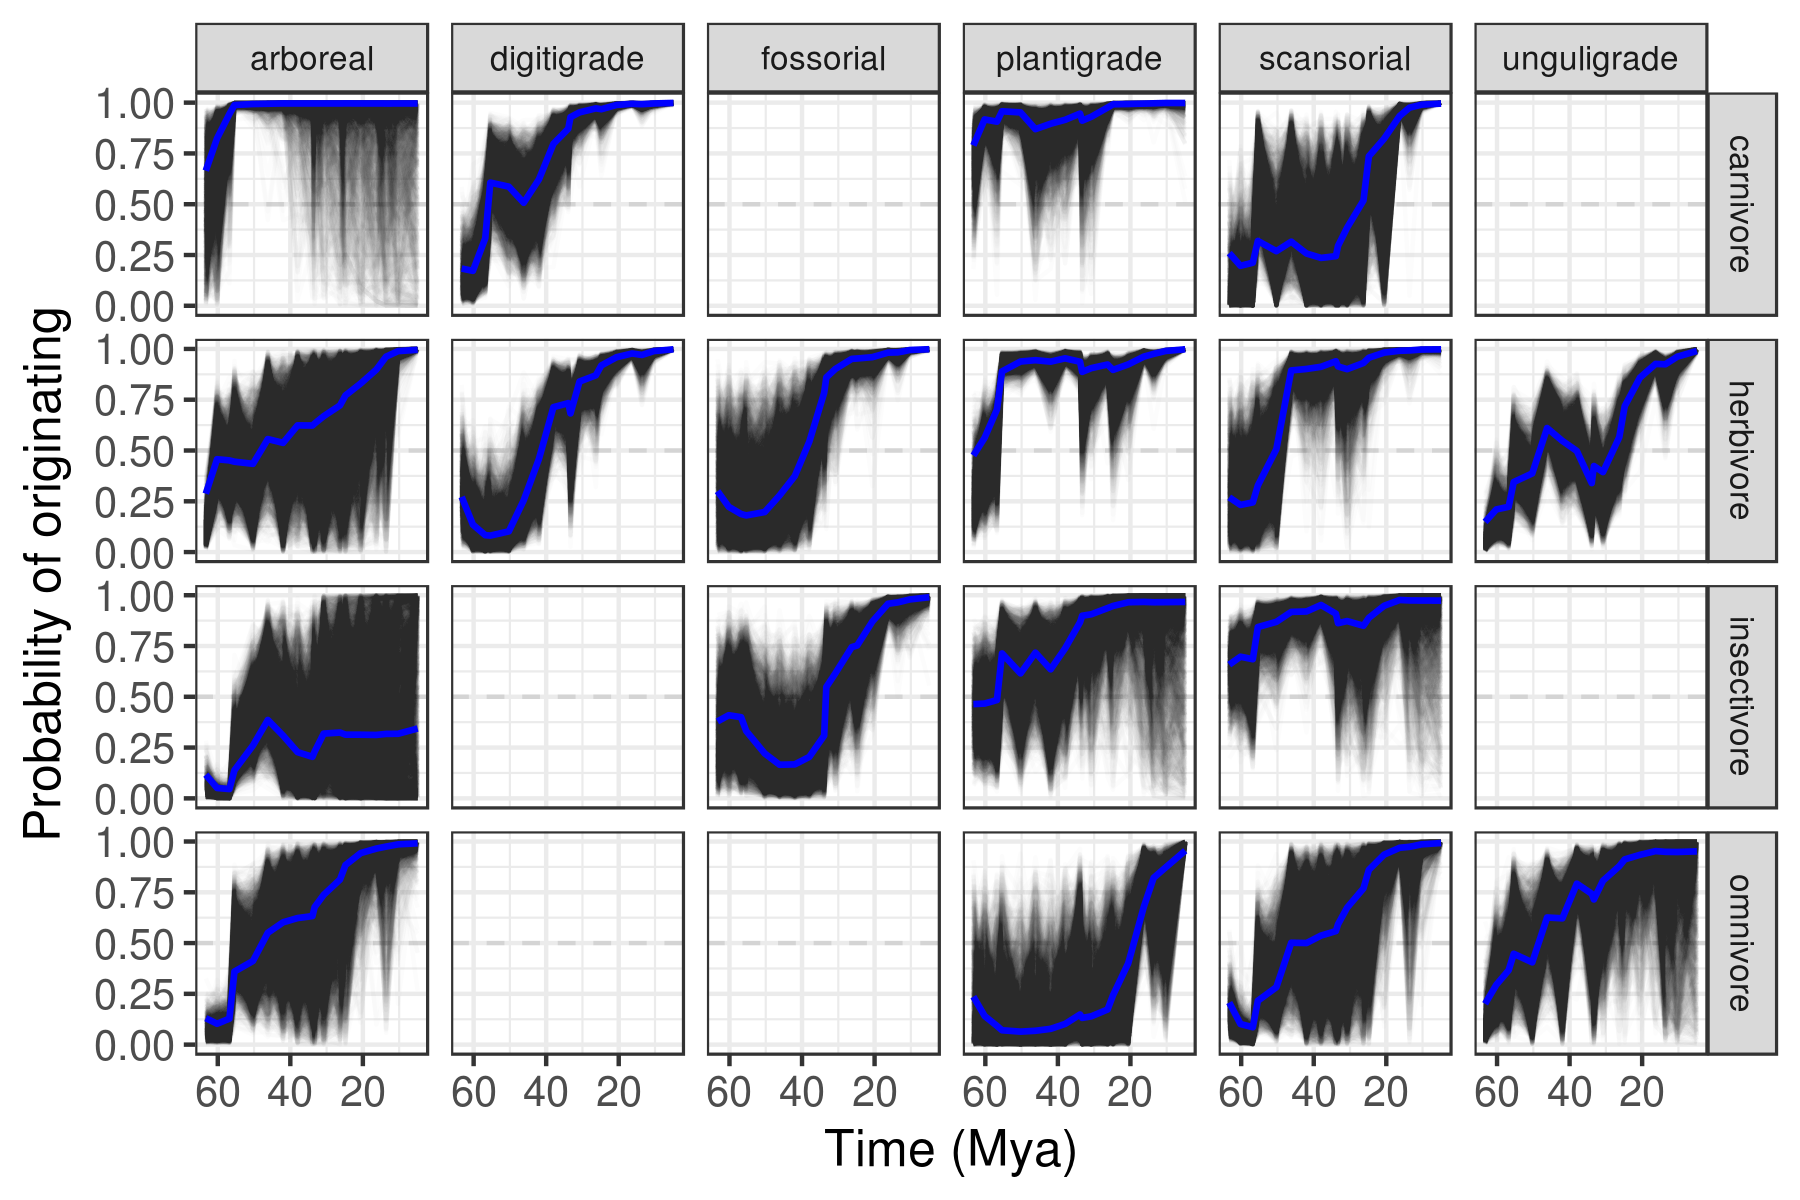
\includegraphics[width=\textwidth,height=0.8\textheight,keepaspectratio=true]{figure/ecotype_origin_bd}
  \caption[Ecotype origination probability estimated from the birth-death model]{Probability of a mammal ecotype origination probabliities at each time point as estimated from the birth-death model. Each panel depicts 100 random samples from the model's posterior. The columns are by locomotor category and rows by dietary category; their intersections are the observed and analyzed ecotypes. Panels with no lines are ecotypes not observed in the dataset.}
  \label{fig:eco_origin}
\end{figure}

\begin{figure}[ht]
  \centering
  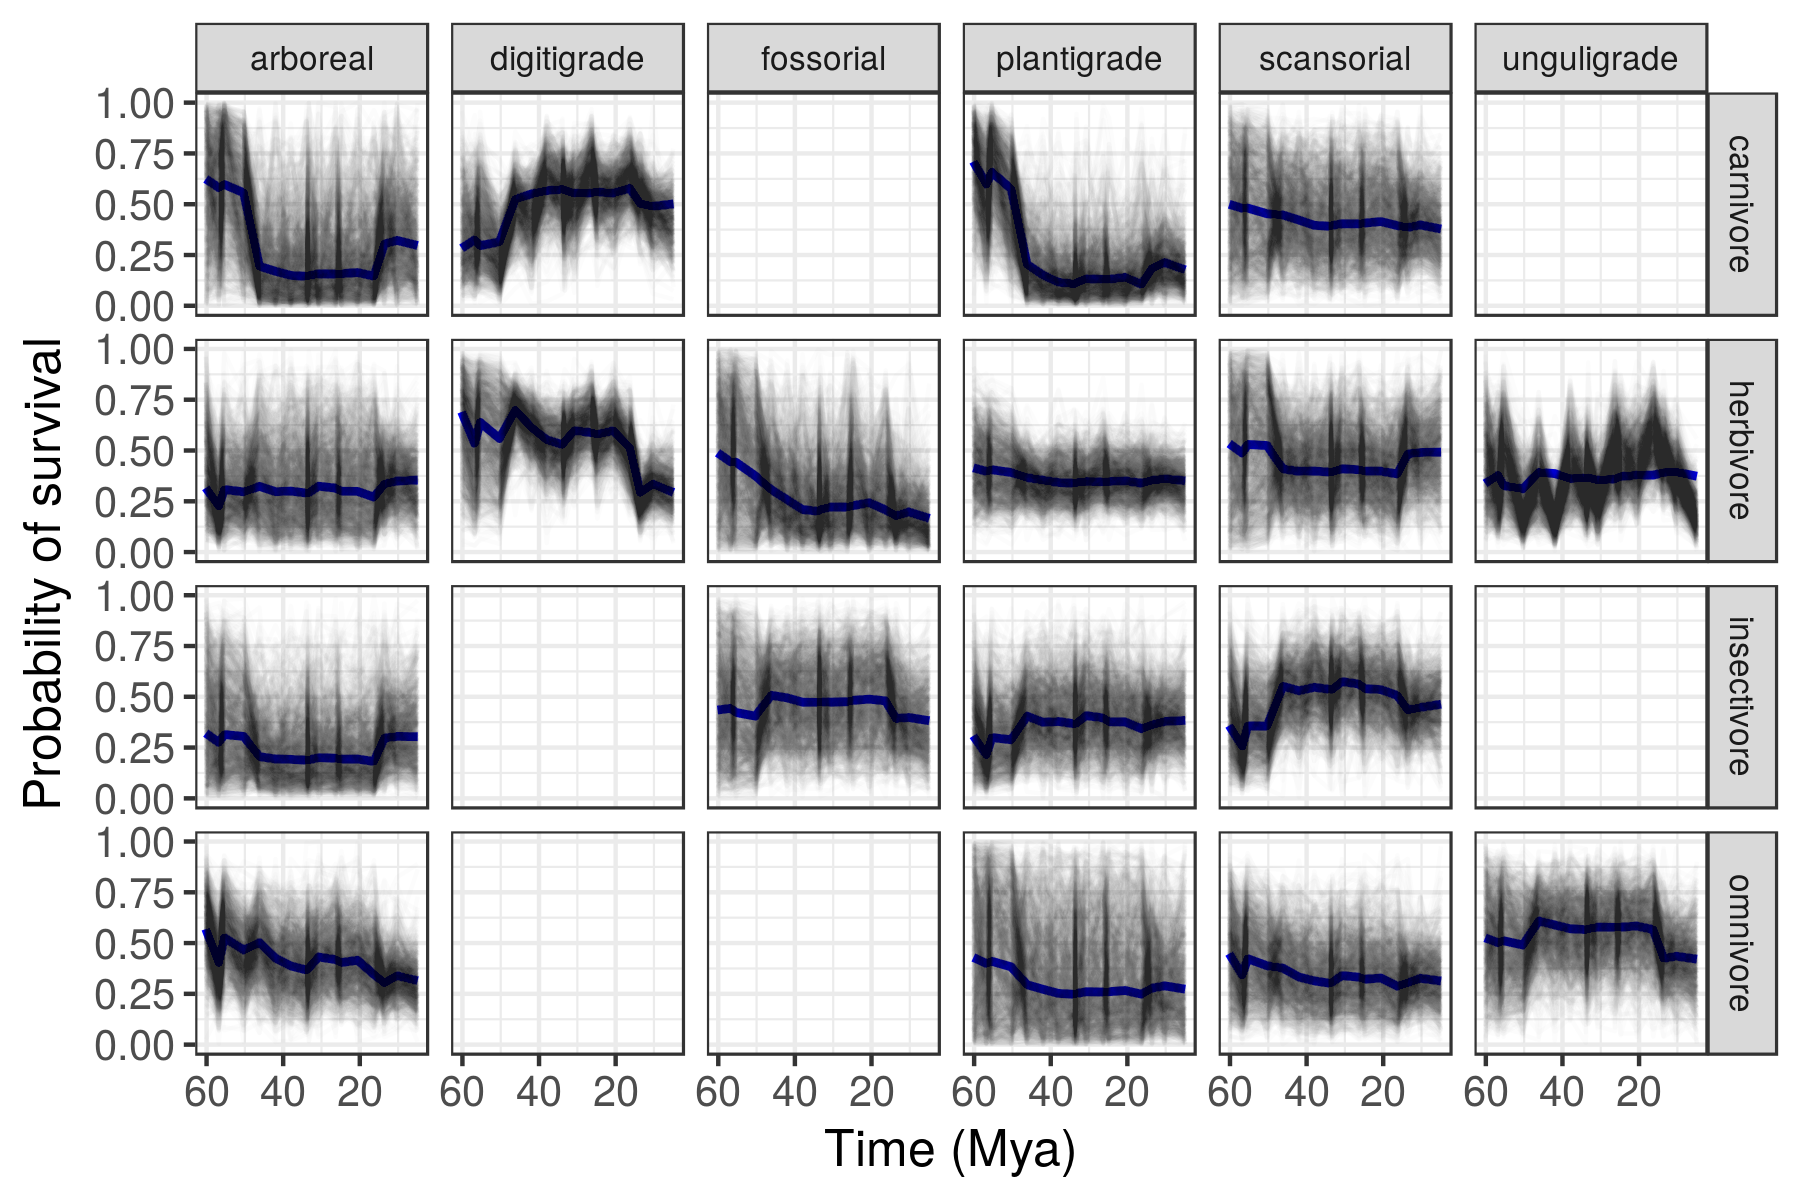
\includegraphics[width=\textwidth,height=0.8\textheight,keepaspectratio=true]{figure/ecotype_survival_bd}
  \caption[Ecotype survival probability estimated from the birth-death model]{Probability of a mammal ecotype survival probabilities at each time point as estimated from the birth-death model. Each panel depicts 100 random samples from the model's posterior. The columns are by locomotor category and rows by dietary category; their intersections are the observed and analyzed ecotypes. Panels with no lines are ecotypes not observed in the dataset.}
  \label{fig:eco_survival}
\end{figure}


For both the pure-presence and birth-death models there appears to be little effect of mass on the probability of observing a present species (Fig. \ref{fig:mass_preserve_pure_pres}, and \ref{fig:mass_preserve_bd}). These results may be unexpected given that it is generally assumed that larger mammals are more likely to have been collected than smaller mammals CITATION. However, collection is not preservation; 


\begin{figure}[ht]
  \centering
  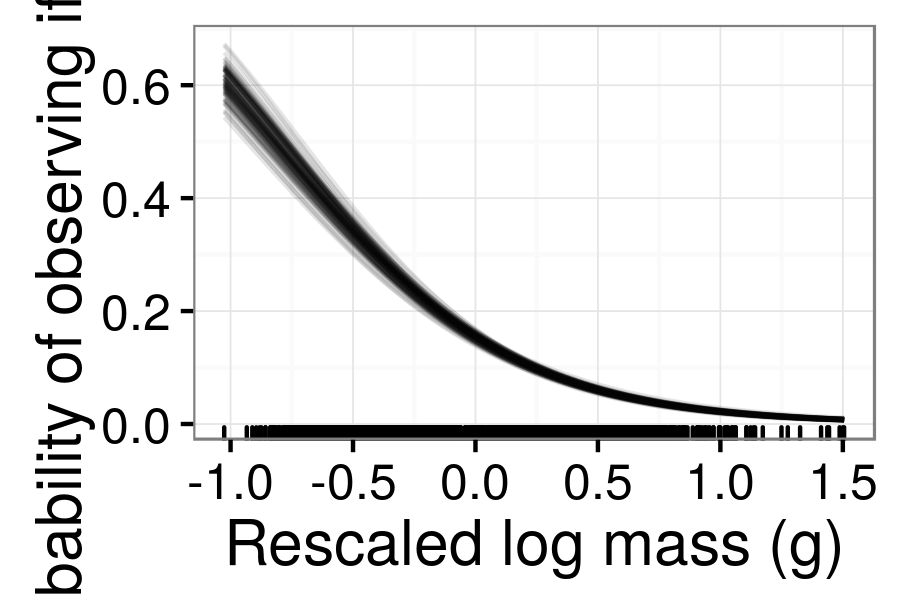
\includegraphics[width=\textwidth,height=0.8\textheight,keepaspectratio=true]{figure/mass_on_samp}
  \caption[Estimates of the effect of mass on observation probability from the pure-presence model]{Estimates of the effect of species mass on probability of observing a present species (\(p\)). Mass has been log-transformed, centered, and rescaled; this means that a mass of 0 corresponds to the mean of log-mass of all observed species and that mass is in standard deviation units. Estimates are from the pure-presence model.}
  \label{fig:mass_preserve_pure_pres}
\end{figure}

\begin{figure}[ht]
  \centering
  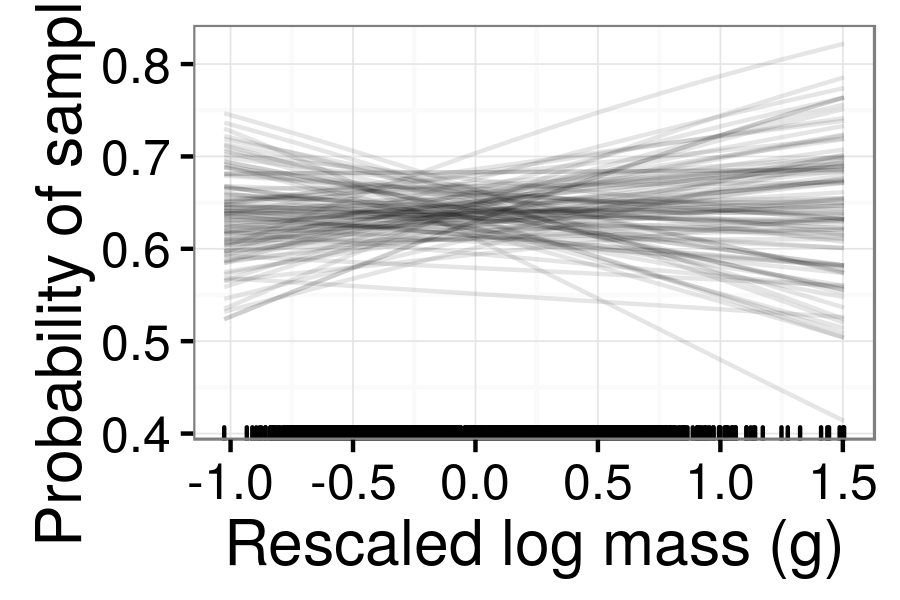
\includegraphics[width=\textwidth,height=0.8\textheight,keepaspectratio=true]{figure/mass_on_samp_bd}
  \caption[Estimates of the effect of mass on observation probability from the birth-death model]{Estimates of the effect of species mass on probability of observing a present species (\(p\)). Mass has been log-transformed, centered, and rescaled; this means that a mass of 0 corresponds to the mean of log-mass of all observed species and that mass is in standard deviation units. Estimates are from the birth-death model.}
  \label{fig:mass_preserve_bd}
\end{figure}

\begin{figure}[ht]
  \centering
  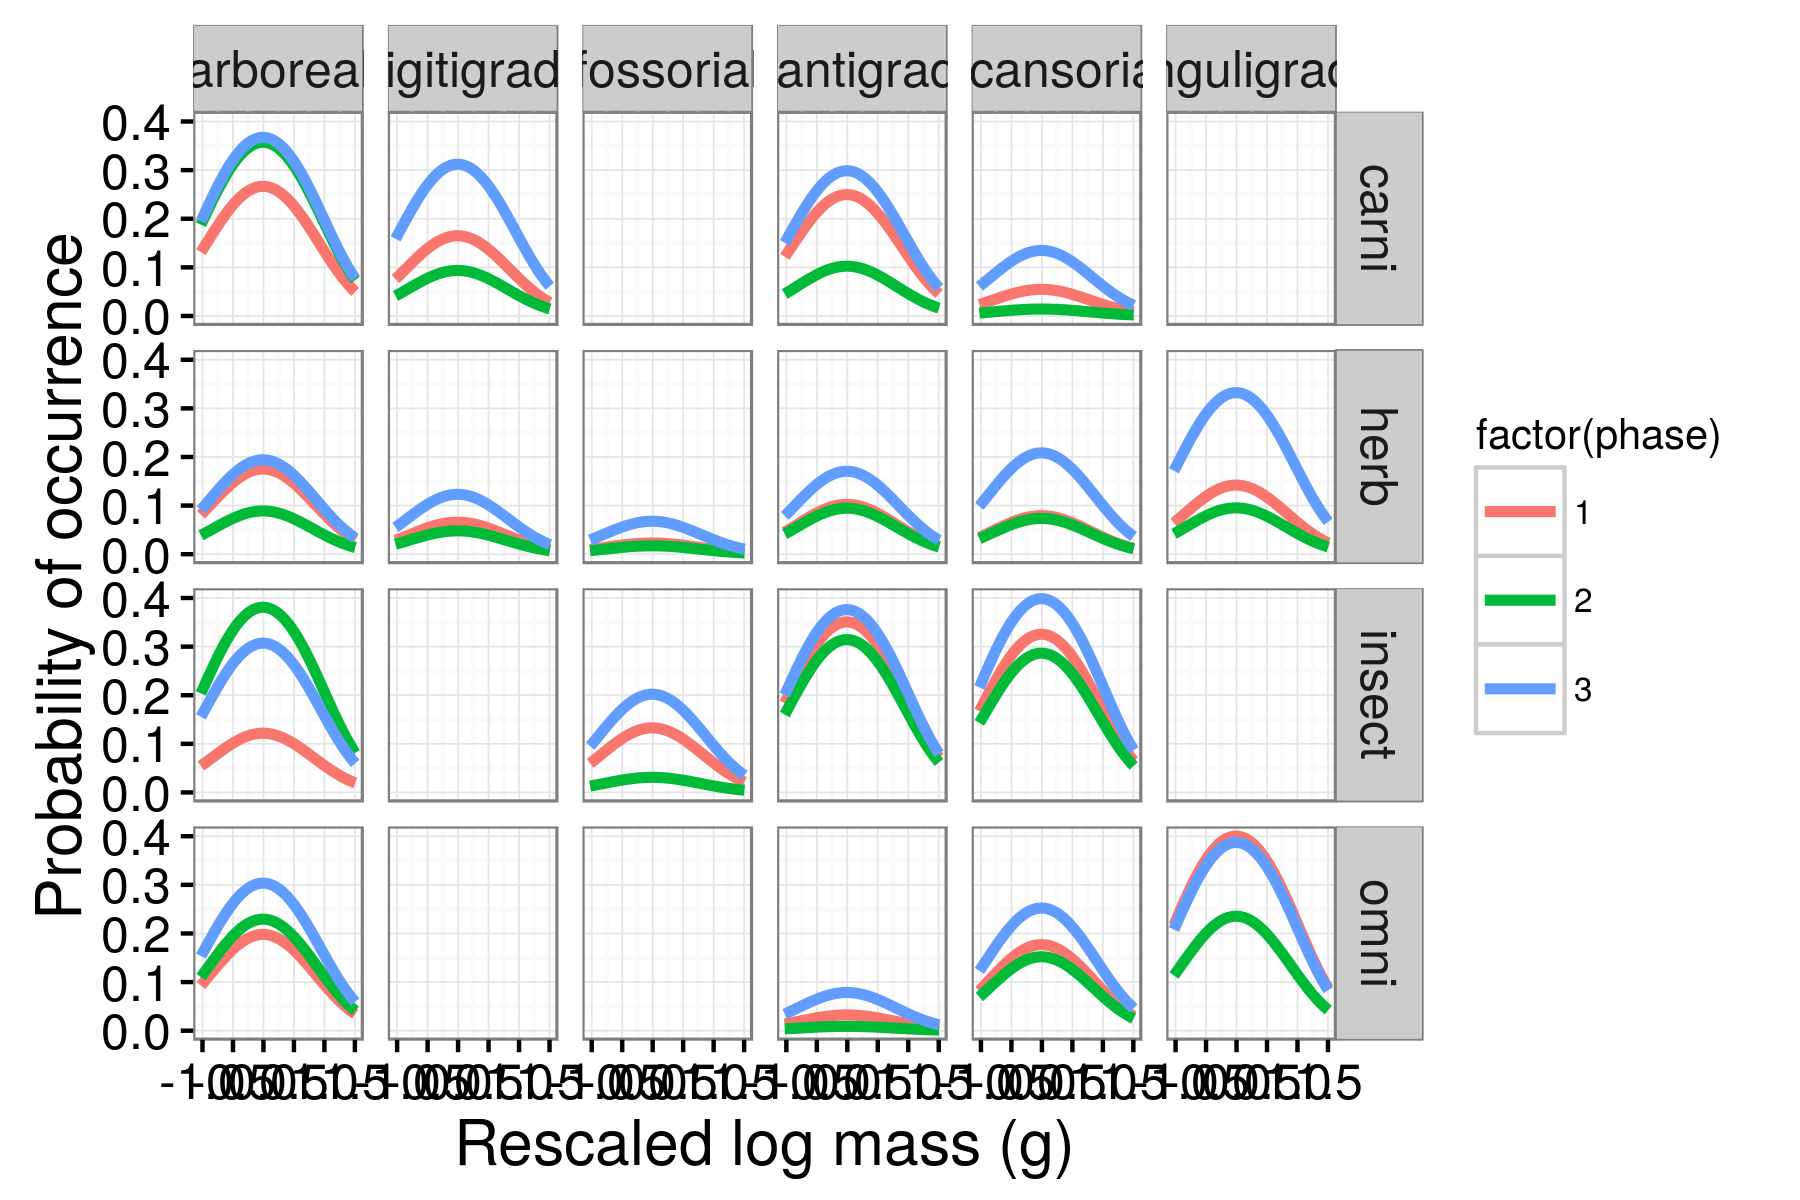
\includegraphics[width=\textwidth,height=0.8\textheight,keepaspectratio=true]{figure/mass_on_pres}
  \caption[Effect of mass on probability of species occurrence as estimated from the pure-presence model]{Mean estimate of the effect of species mass on the probability of a species occurrence for each of the three plant phases. The effect of mass is considered constant over time and that the only aspect of the model that changes with plant phase is the intercept of the relationship between mass and occurrence. The three plant phases are indicated by the color of the line. Mass has been log-transformed, centered, and rescaled; this means that a mass of 0 corresponds to the mean of log-mass of all observed species and that mass is in standard deviation units.}
  \label{fig:mass_occur}
\end{figure}

\begin{figure}[ht]
  \centering
  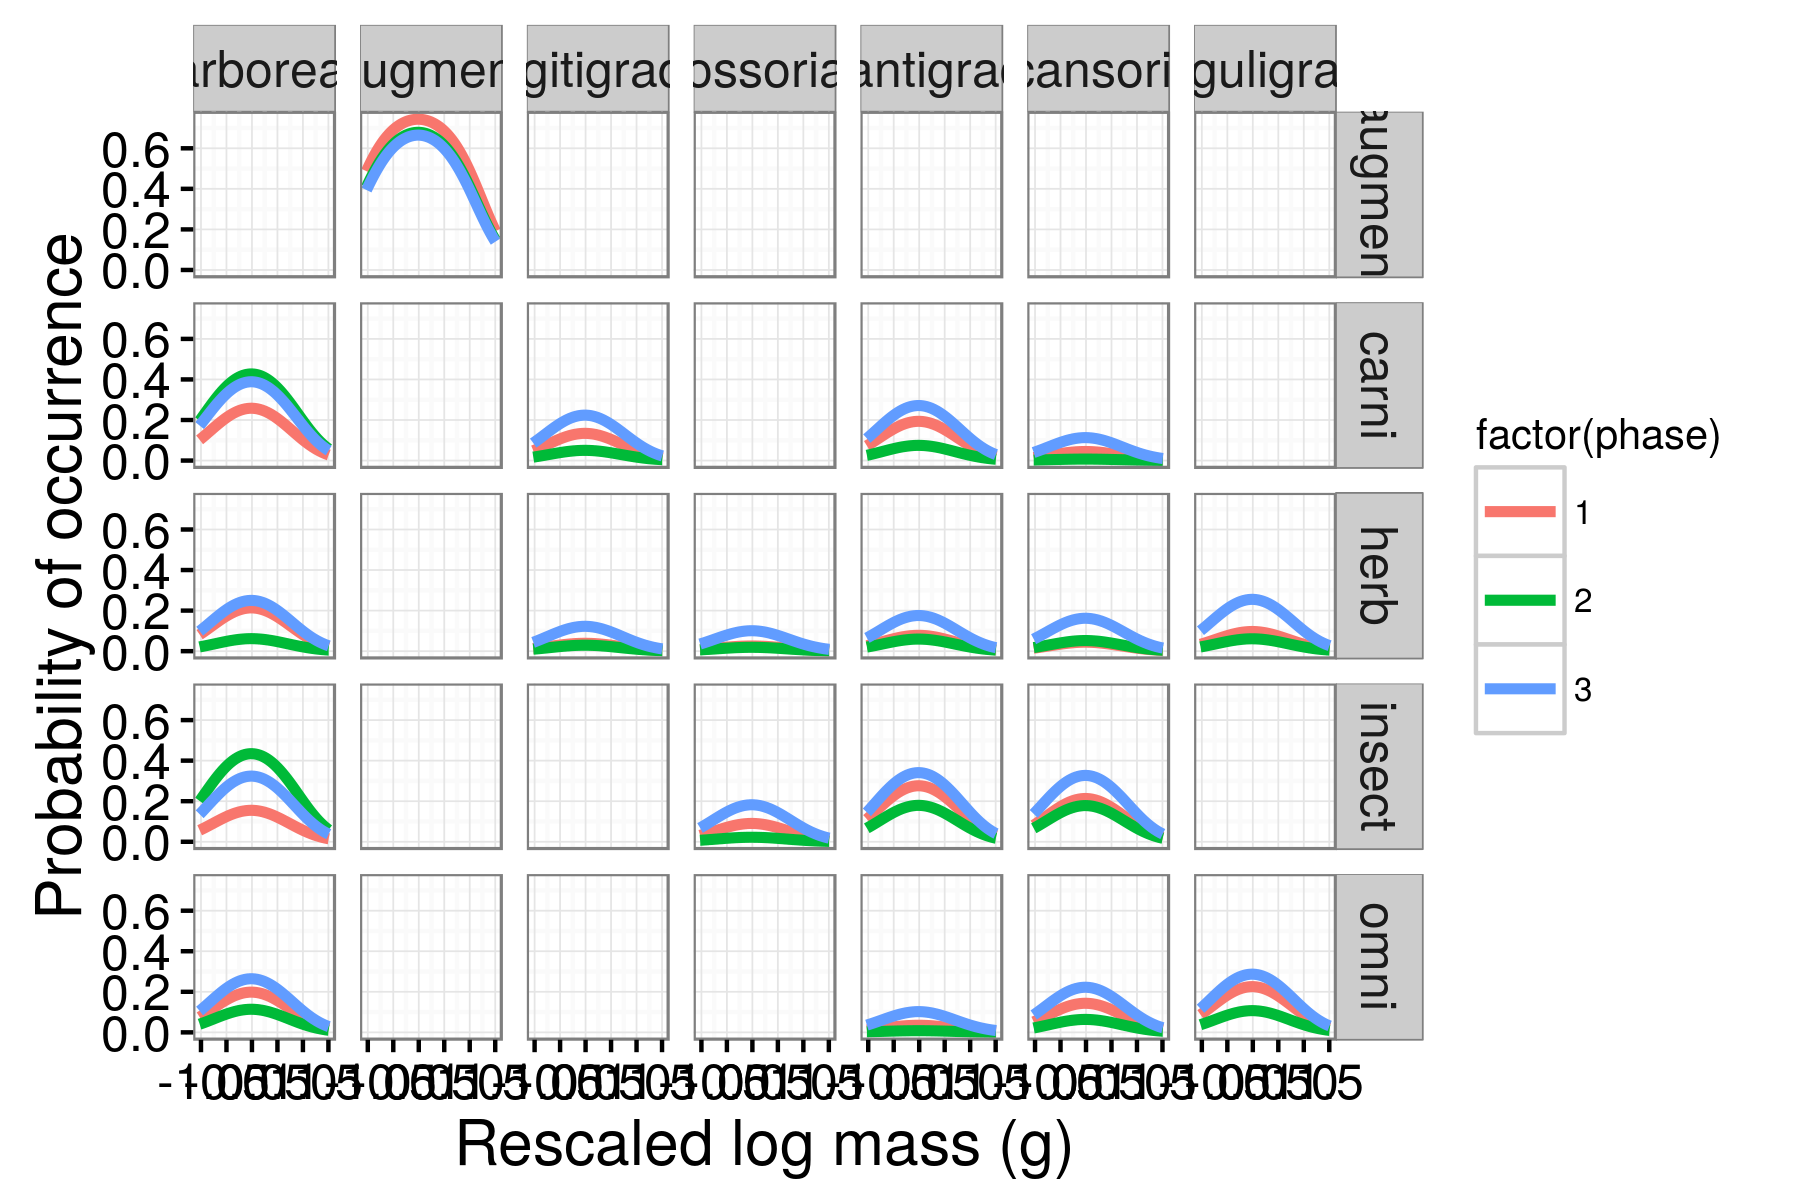
\includegraphics[width=\textwidth,height=0.8\textheight,keepaspectratio=true]{figure/mass_on_origin_bd}
  \caption[Effect of mass on probability of species origination as estimated from the birth-death model]{Mean estimate of the effect of species mass on the probability of a species originating for each of the three plant phases. The effect of mass is considered constant over time and that the only aspect of the model that changes with plant phase is the intercept of the relationship between mass and origination. The three plant phases are indicated by the color of the line. Mass has been log-transformed, centered, and rescaled; this means that a mass of 0 corresponds to the mean of log-mass of all observed species and that mass is in standard deviation units.}
  \label{fig:mass_origin}
\end{figure}

\begin{figure}[ht]
  \centering
  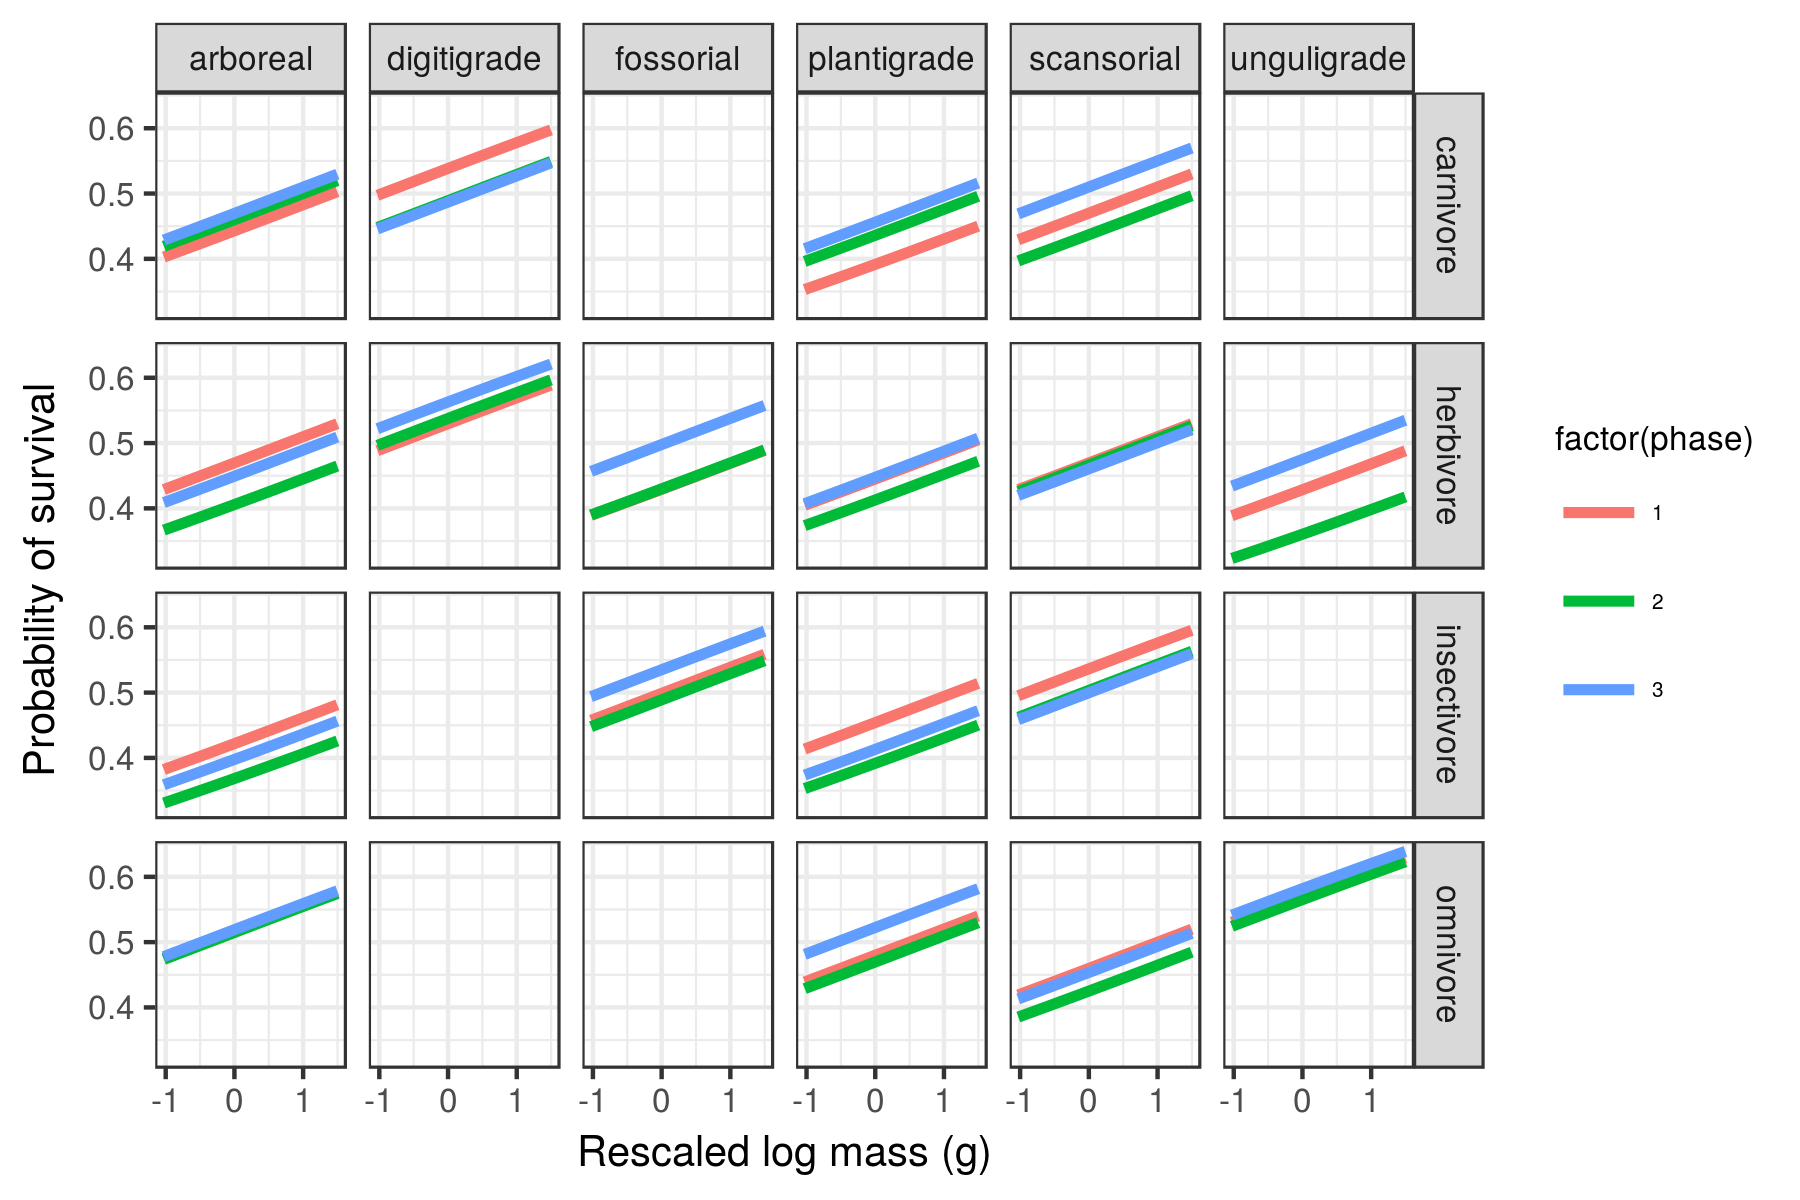
\includegraphics[width=\textwidth,height=0.8\textheight,keepaspectratio=true]{figure/mass_on_surv_bd}
  \caption[Effect of mass on probability of species survival as estimated from the birth-death model]{Mean estimate of the effect of species mass on the probability of a species survival for each of the three plant phases. The effect of mass is considered constant over time and that the only aspect of the model that changes with plant phase is the intercept of the relationship between mass and survival. The three plant phases are indicated by the color of the line. Mass has been log-transformed, centered, and rescaled; this means that a mass of 0 corresponds to the mean of log-mass of all observed species and that mass is in standard deviation units.}
  \label{fig:mass_survival}
\end{figure}

\begin{figure}[ht]
  \centering
  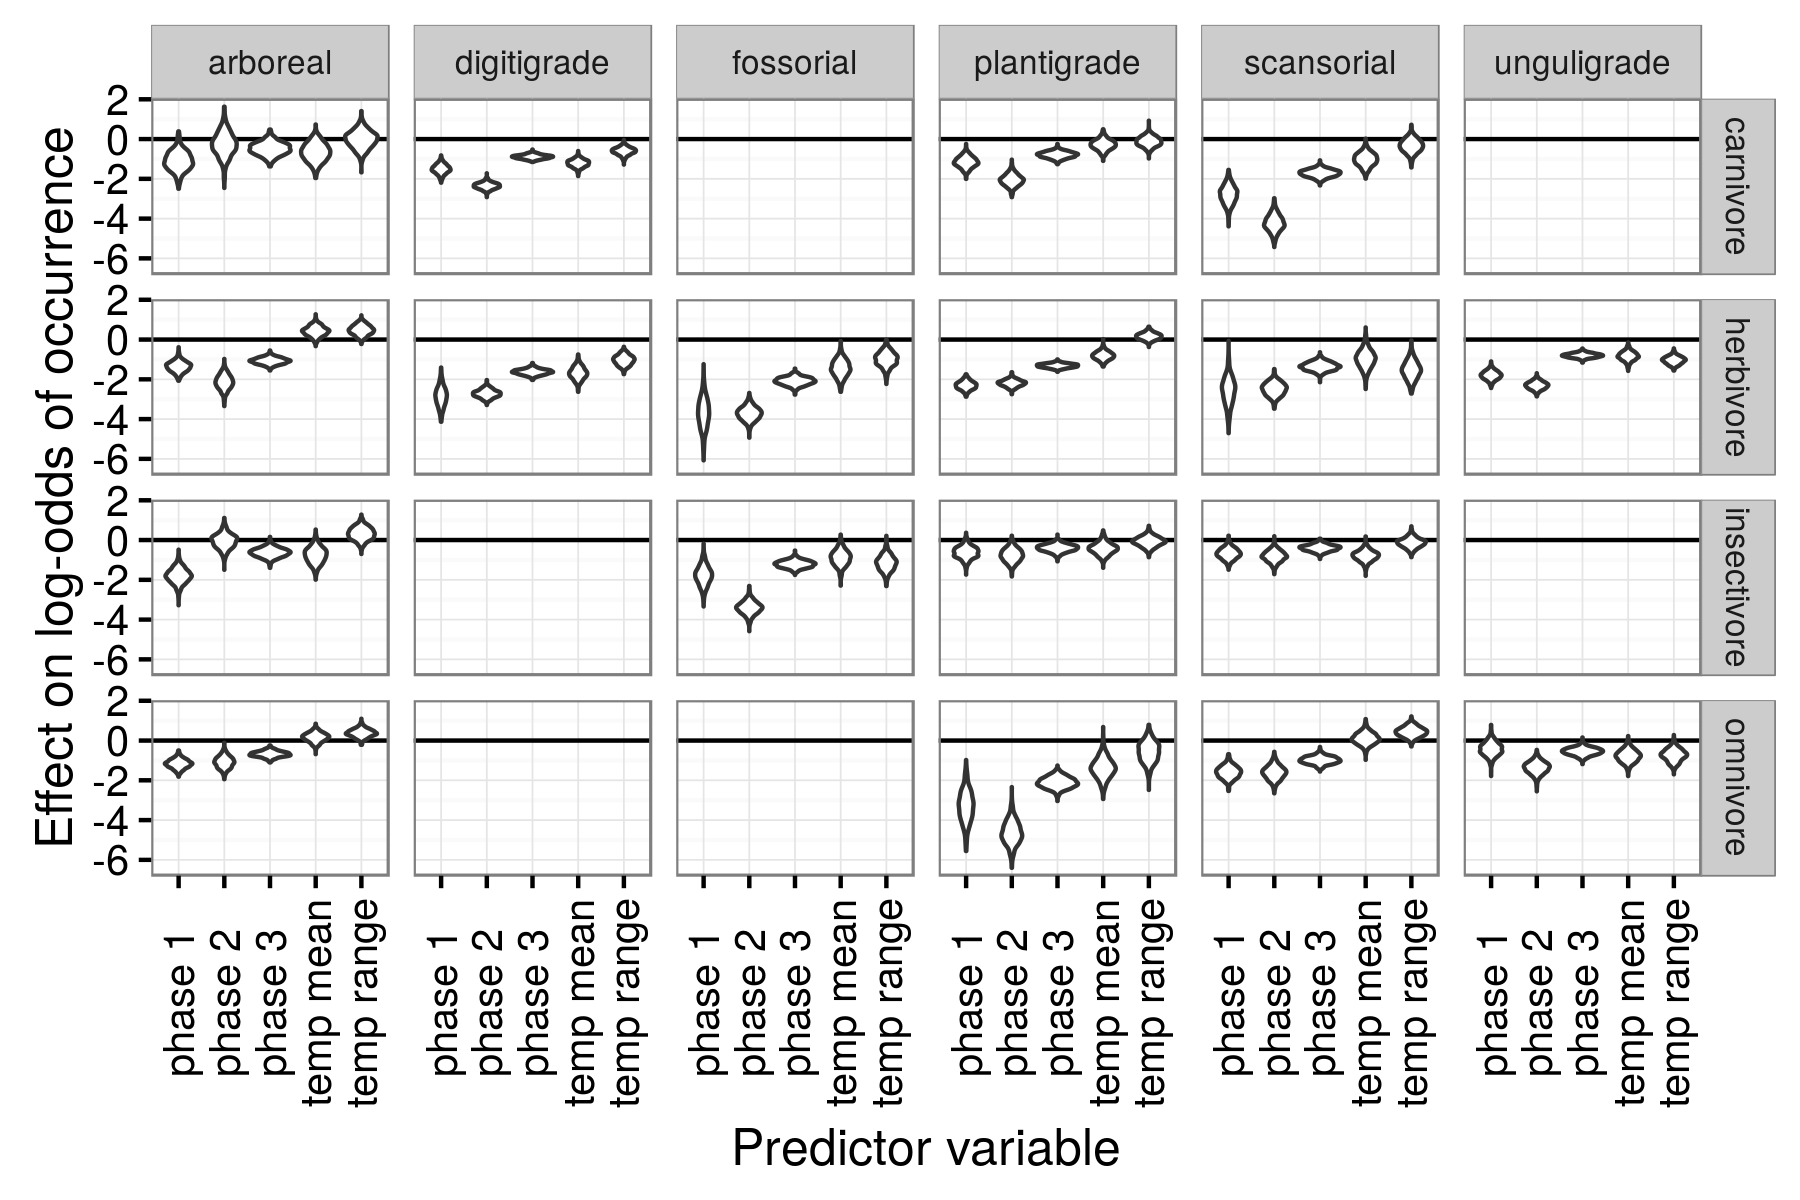
\includegraphics[width=\textwidth,height=0.8\textheight,keepaspectratio=true]{figure/group_on_ecotype}
  \caption[Effects of group-level covariates on log-odds of ecotype occurrence as estimated from the the pure-presence model]{Estimated effects of the group-level covariates describing environmental context on log-odds of species occurrence. These estimates are from the pure-presence model.} 
  \label{fig:group_pure_presence}
\end{figure}

\begin{figure}[ht]
  \centering
  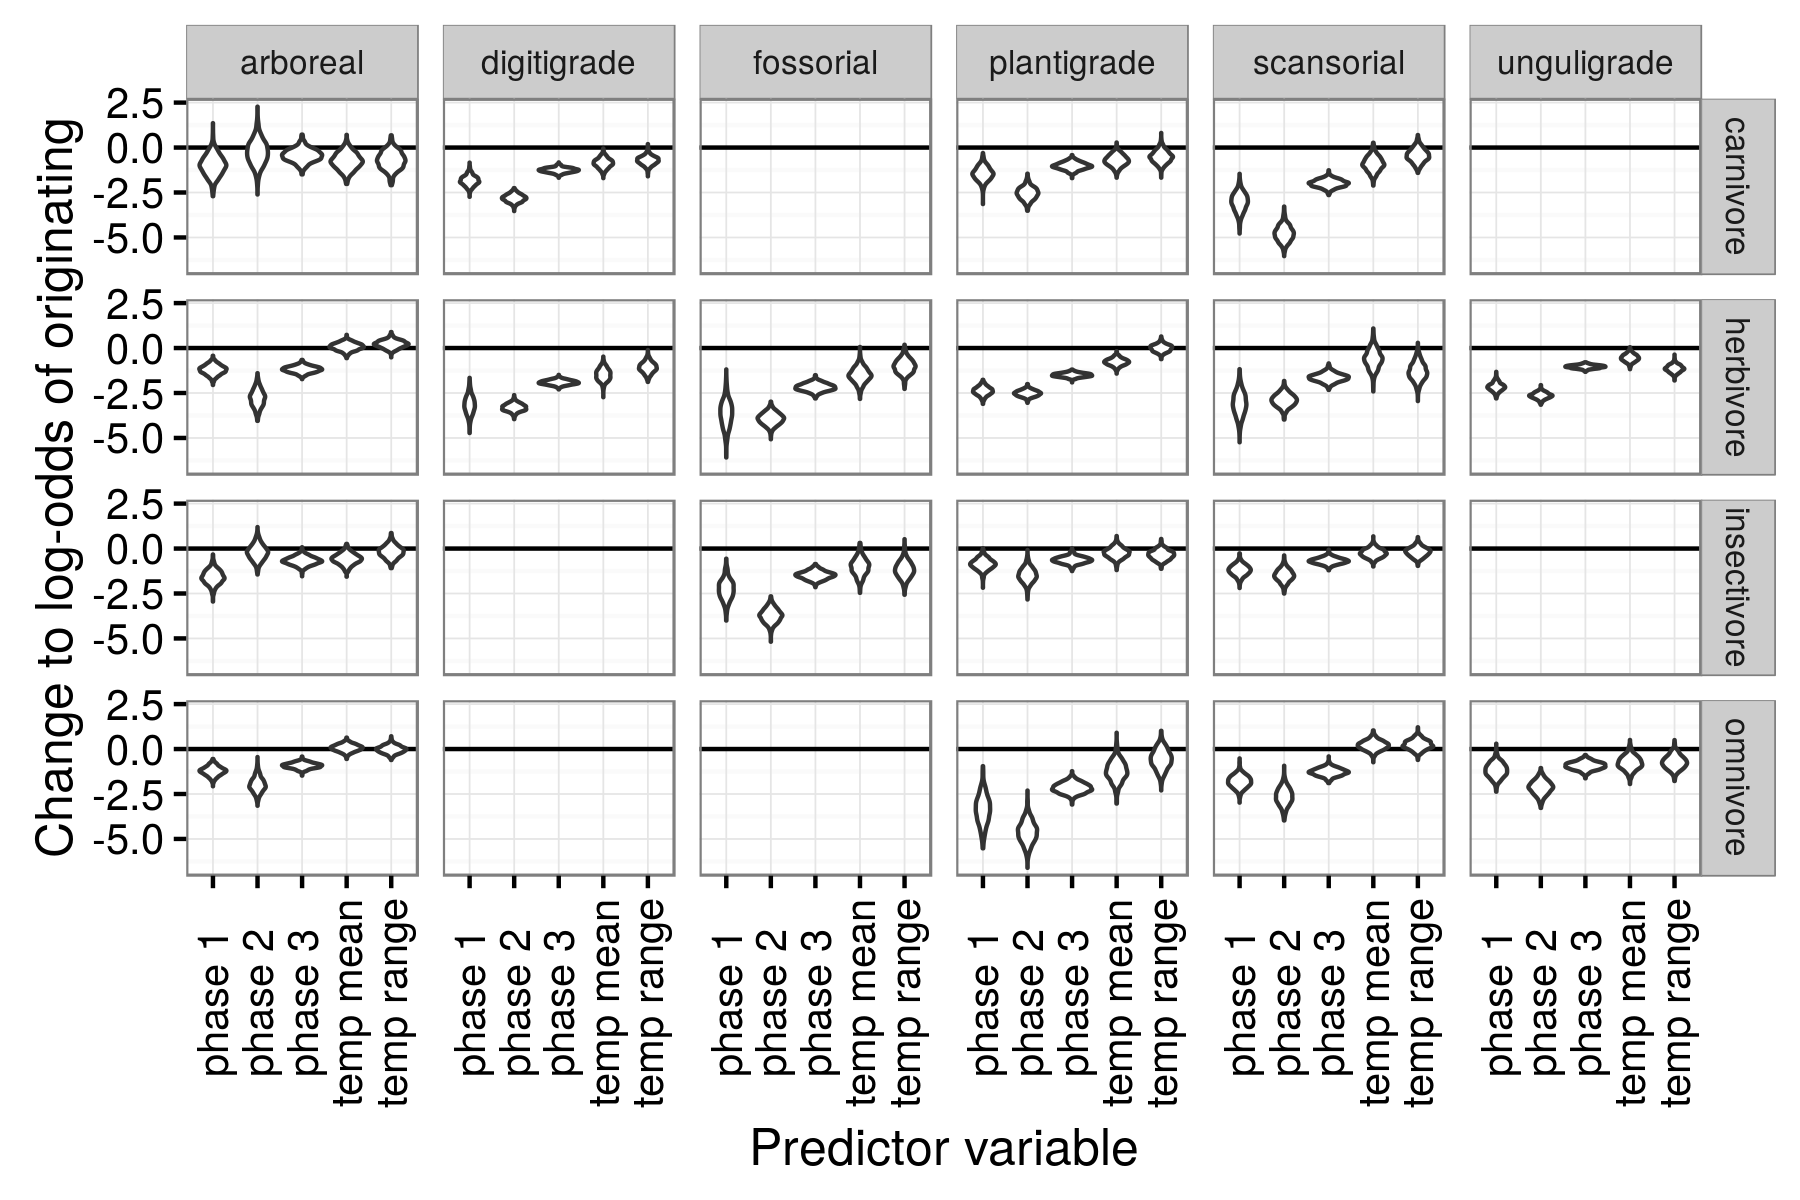
\includegraphics[width=\textwidth,height=0.8\textheight,keepaspectratio=true]{figure/group_on_origin_bd}
  \caption[Effects of group-level covariates on log-odds of ecotype origination as estimated from the the birth-death model]{Estimated effects of the group-level covariates describing environmental context on log-odds of species origination. These estimates are from the birth-death model.}
  \label{fig:group_origin_bd}
\end{figure}

\begin{figure}[ht]
  \centering
  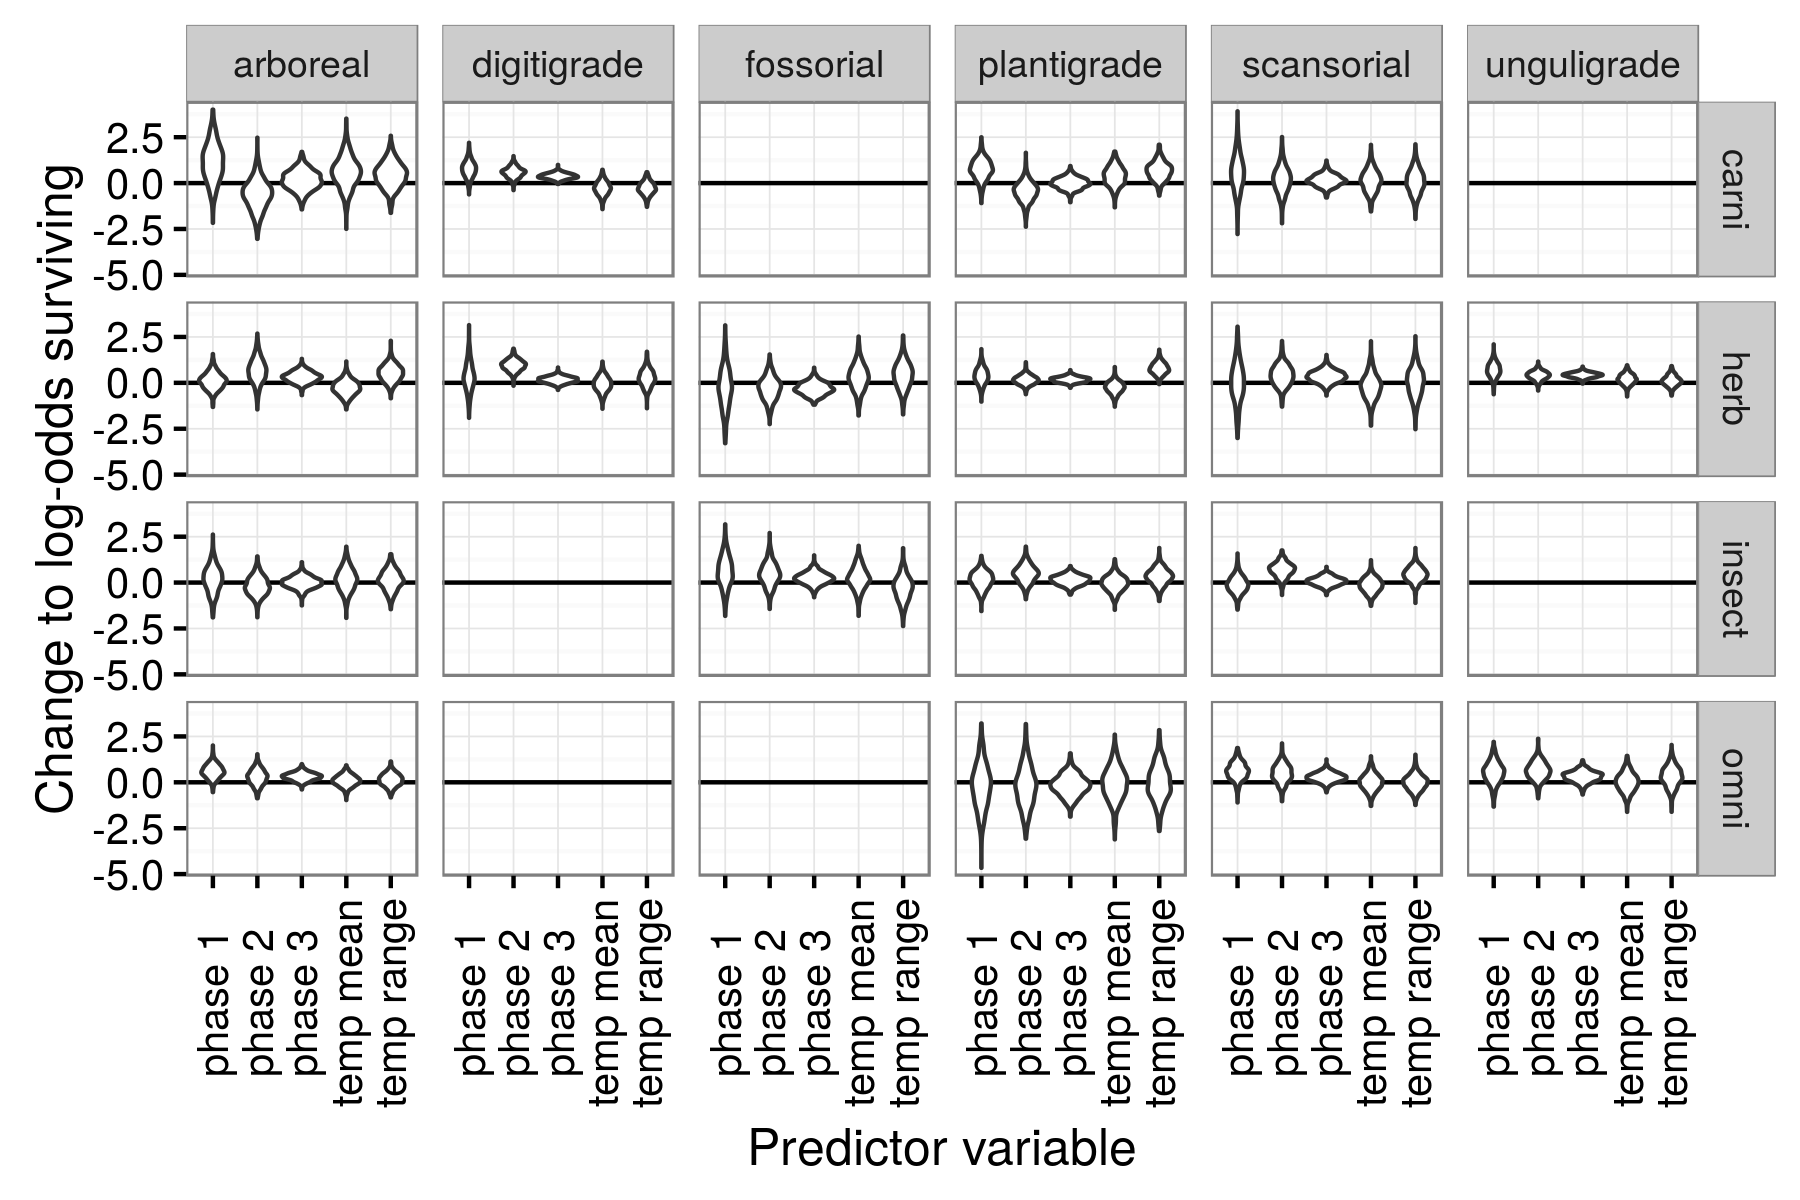
\includegraphics[width=\textwidth,height=0.8\textheight,keepaspectratio=true]{figure/group_on_survival_bd}
  \caption[Effects of group-level covariates on log-odds of ecotype survival as estimated from the the birth-death model]{Estimated effects of the group-level covariates describing environmental context on log-odds of species survlval. These estimates are from the birth-death model.}
  \label{fig:group_surv_bd}
\end{figure}


\subsection*{Analysis of diversity}
\begin{figure}[ht]
  \centering
  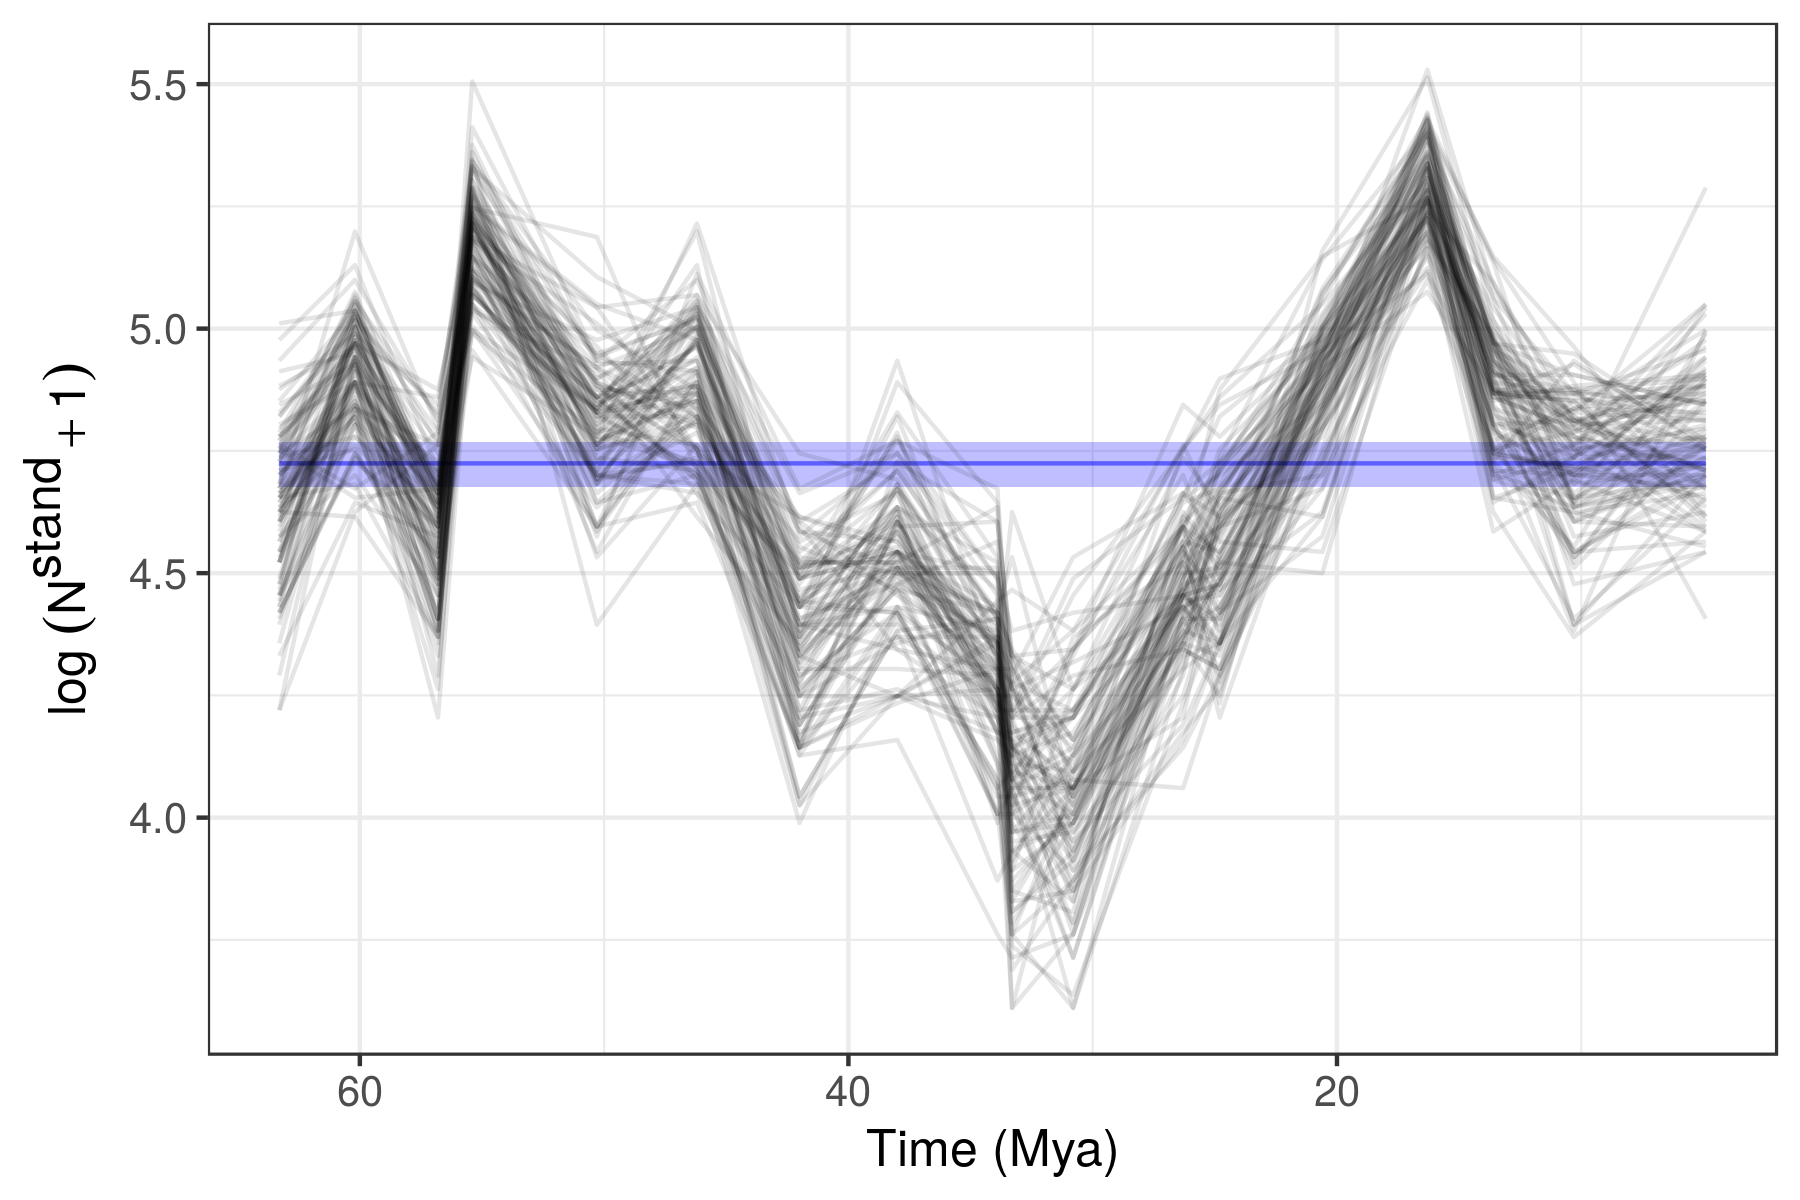
\includegraphics[width=\textwidth,height=0.8\textheight,keepaspectratio=true]{figure/log_diversity}
  \caption[Estimated mammal log-diversity for the Cenozoic]{Posterior of standing log-diversity of North American mammals for the Cenozoic as estimated from the birth-death model; 100 posterior draws are plotted to indicate the uncertainty in these estimates and what is technically plotted is log of diversity plus 1. The dramatic differences between diversity estimates at the first and second time points and the penultimate and last time points in this series are caused by well known edge effects in discrete-time birth-death models caused by \(p_{\_, t = 1}\) and \(p_{\_, t = T}\) being partially unidentifiable \citep{Royle2008}; the hierarchical modeling strategy used here helps mitigate these effects but they are still present \citep{Gelman2013d,Royle2008}.}
  \label{fig:diversity_est}
\end{figure}

\begin{figure}[ht]
  \centering
  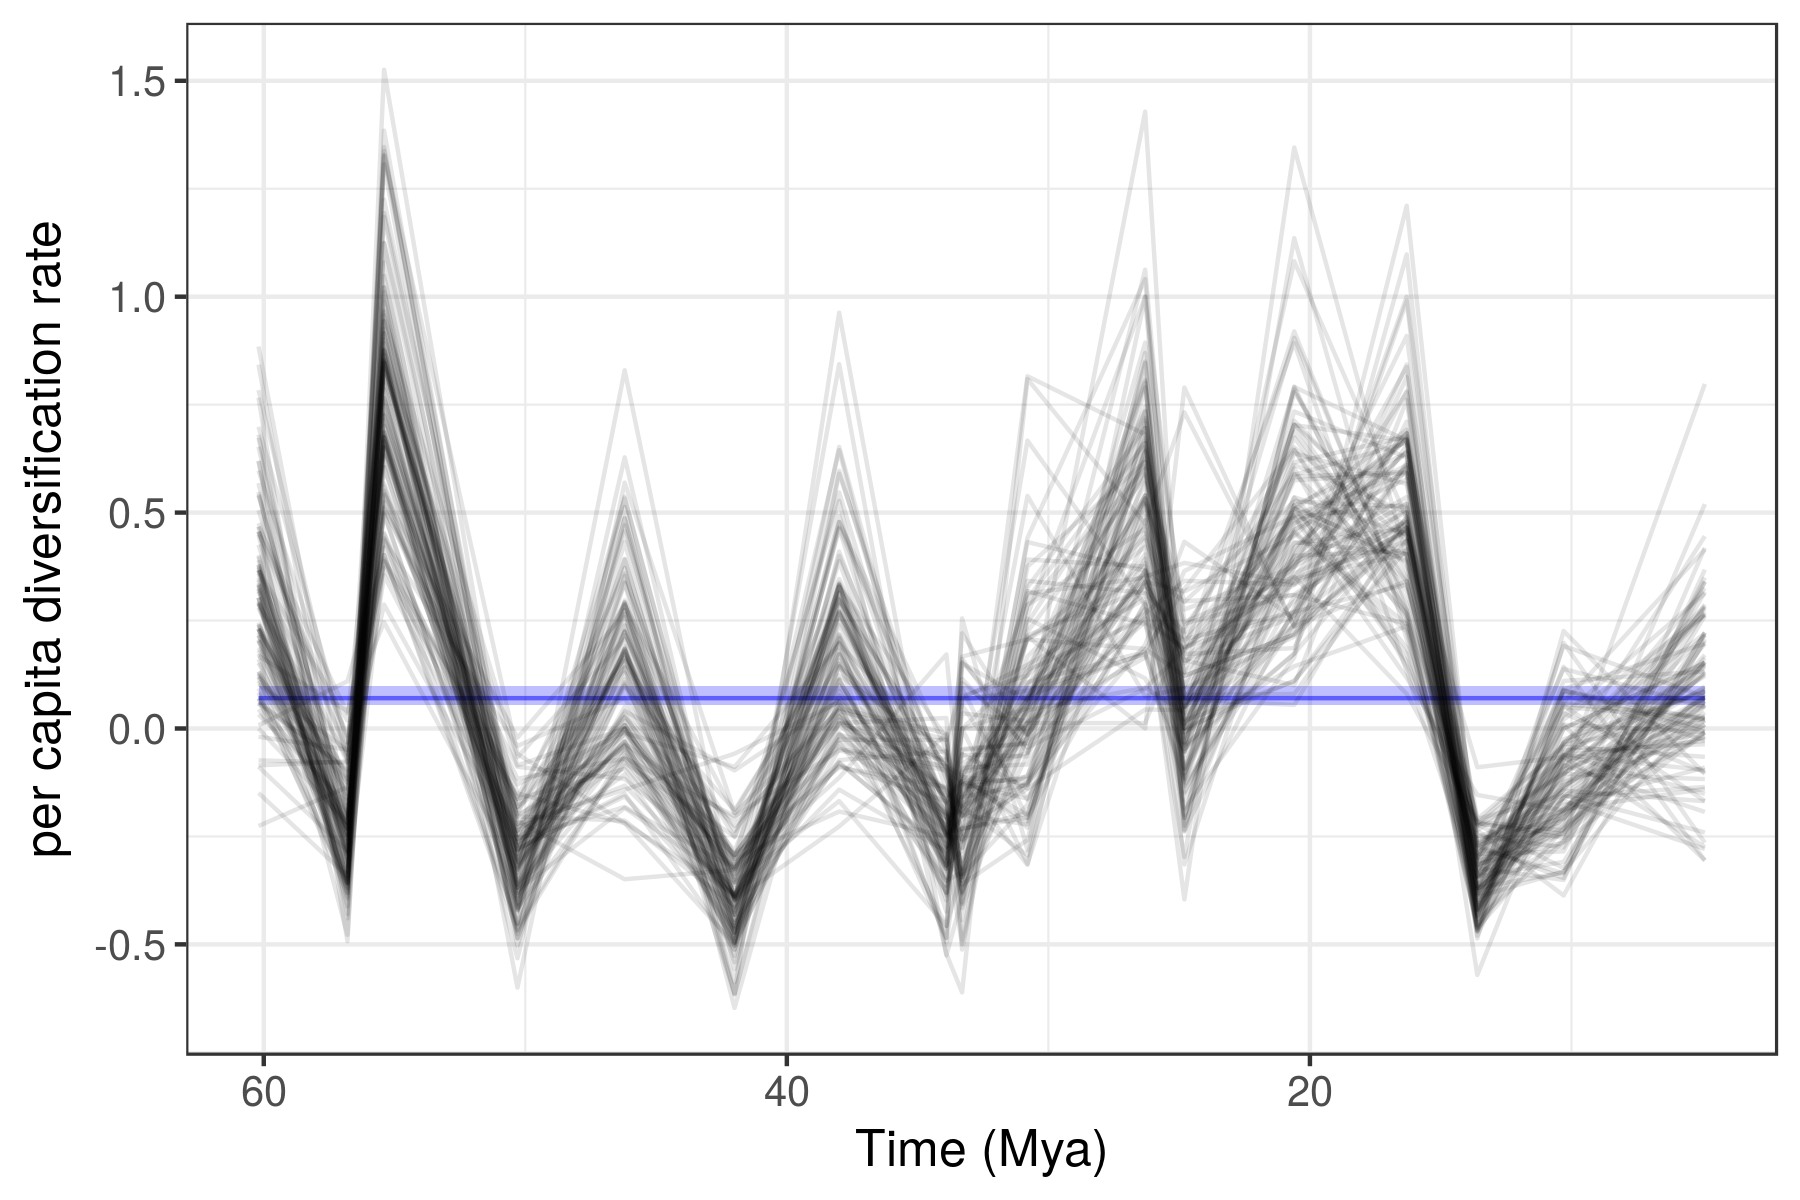
\includegraphics[width=\textwidth,height=0.8\textheight,keepaspectratio=true]{figure/div_rate}
  \caption[Mammal diversification rate estimates]{Posterior estimates of North American mammal diversification rate for the Cenozoic; 100 estimates are plotted to indicate the uncertainty in these estimates. As a reminder, diversification rate is the difference between origination and extinction rates and is in units of species gained per species present per time unit (2 My).}
  \label{fig:diversity_rate}
\end{figure}

\begin{figure}[ht]
  \centering
  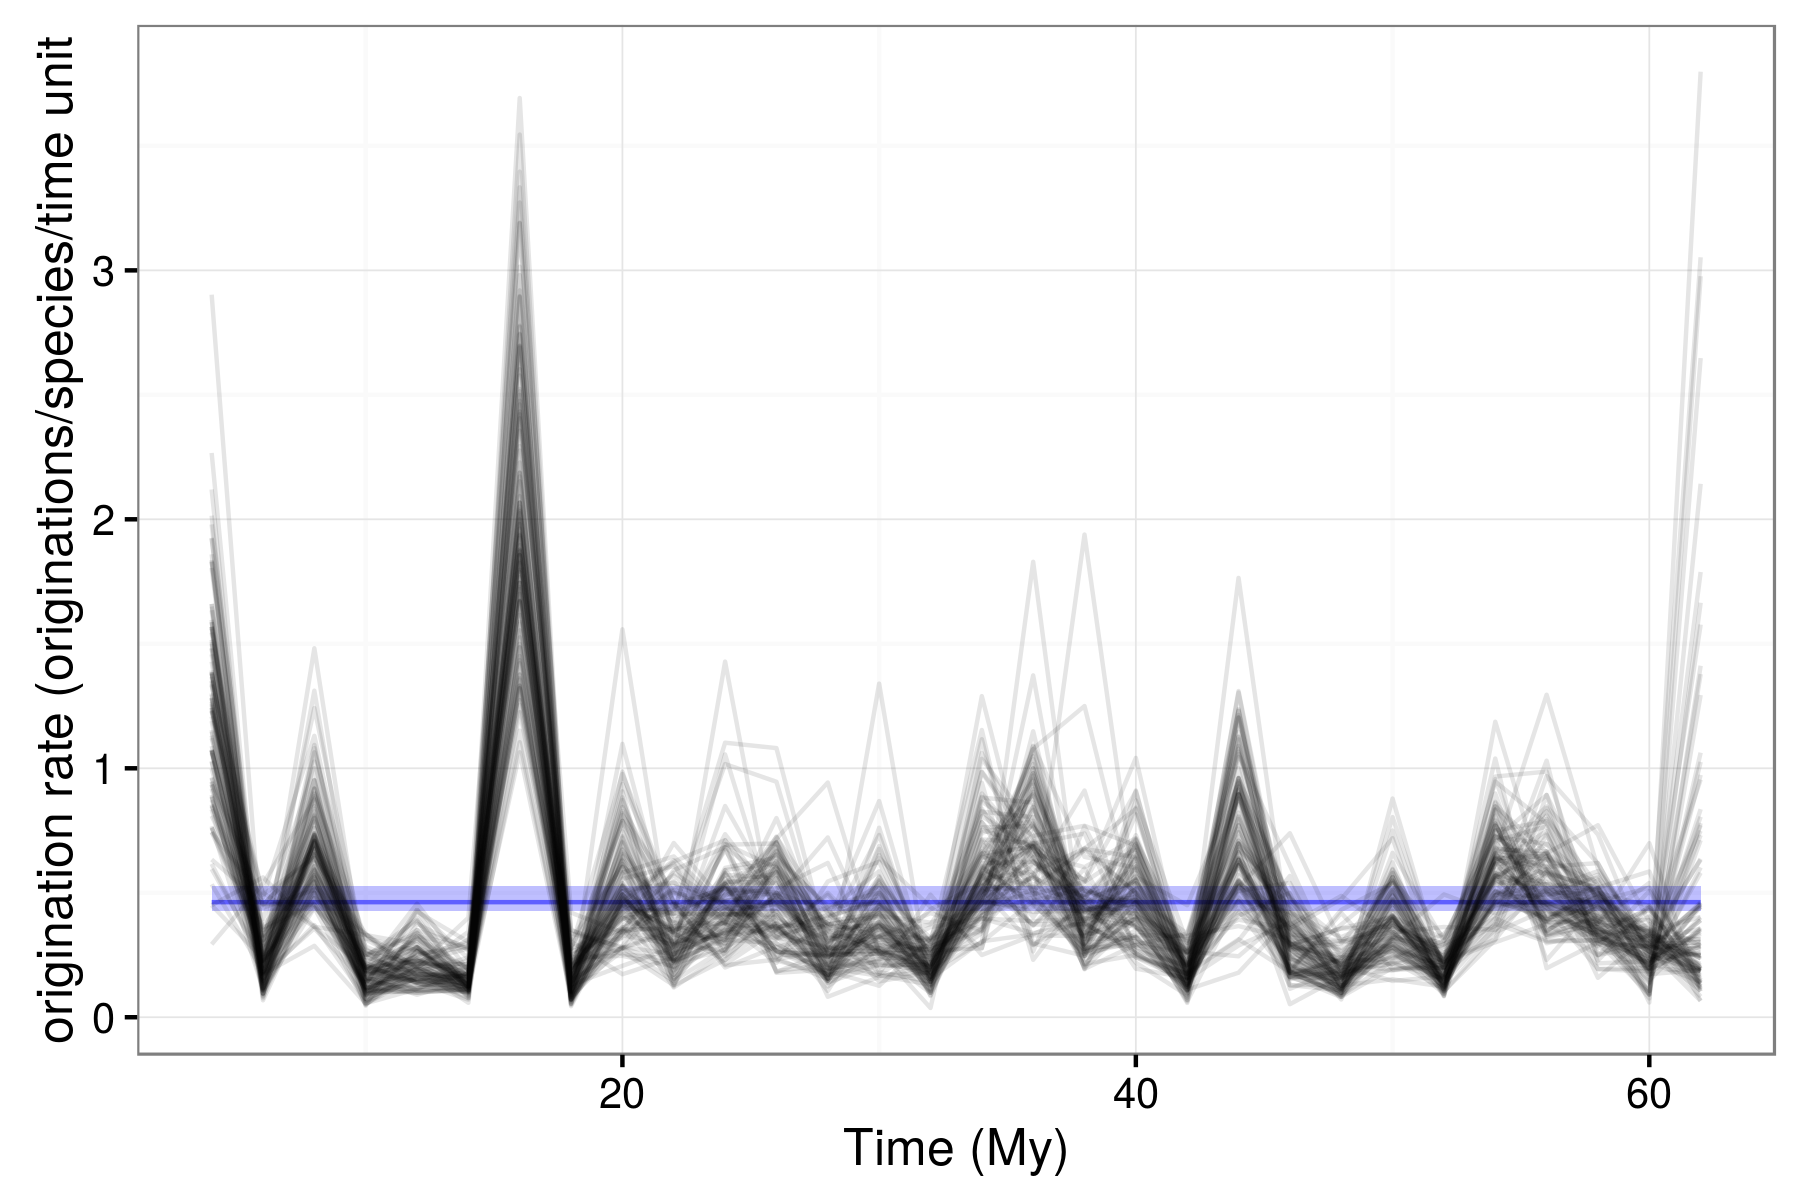
\includegraphics[width=\textwidth,height=0.8\textheight,keepaspectratio=true]{figure/orig_rate}
  \caption[Mammal origination rate estimates]{Posterior estimates of North American origination rate for the Cenozoic; 100 estimates are plotted to indicate the uncertainty in these estimates. The unit of origination rate is number of species originating per species per time unit (2 My).}
  \label{fig:origin_rate}
\end{figure}

\begin{figure}[ht]
  \centering
  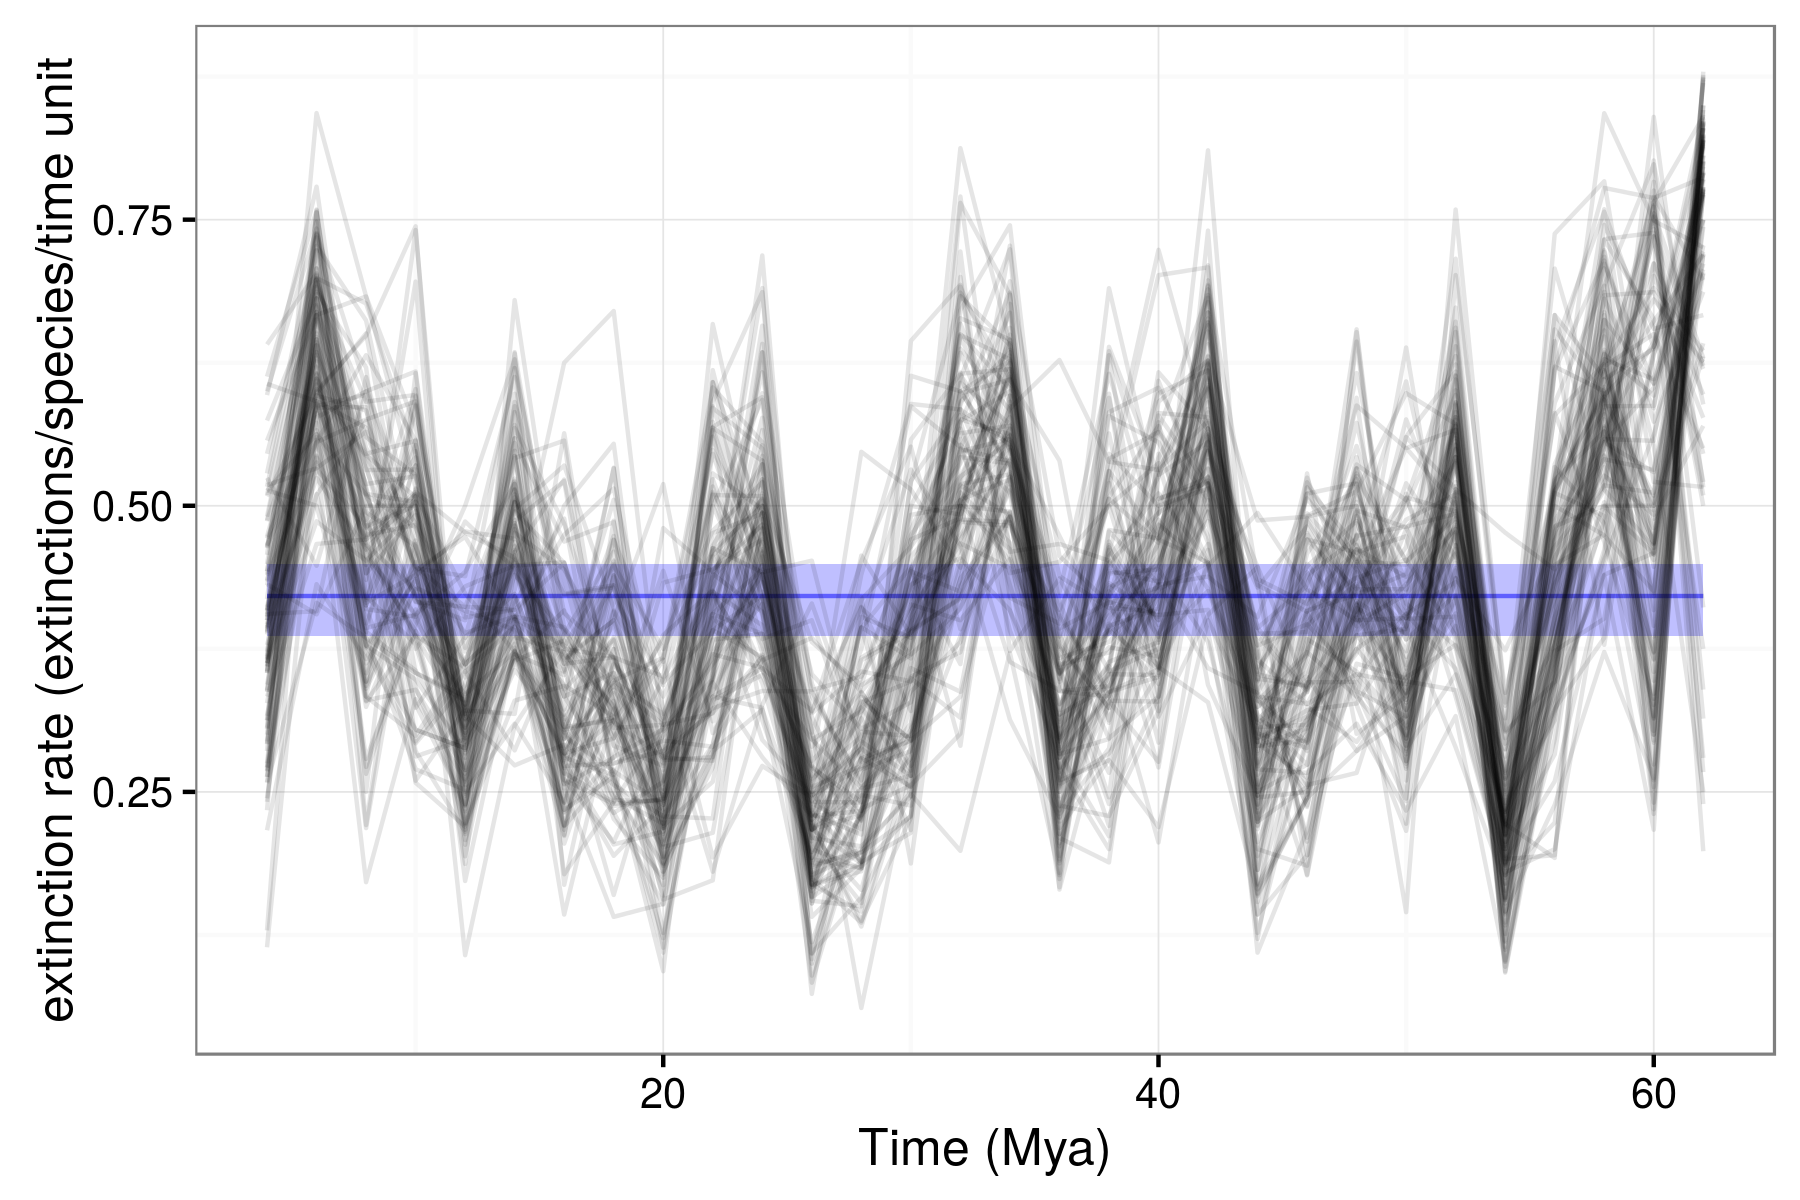
\includegraphics[width=\textwidth,height=0.8\textheight,keepaspectratio=true]{figure/death_rate}
  \caption[Mammal extinction rate estimates]{Posterior estimates of North American extinction rate for the Cenozoic; 100 estimates are plotted to indicate the uncertainty in these estimates. The unit of extinction rate is number of species becoming extinct per species per time unit (2 My).}
  \label{fig:extinct_rate}
\end{figure}

\begin{figure}[ht]
  \centering
  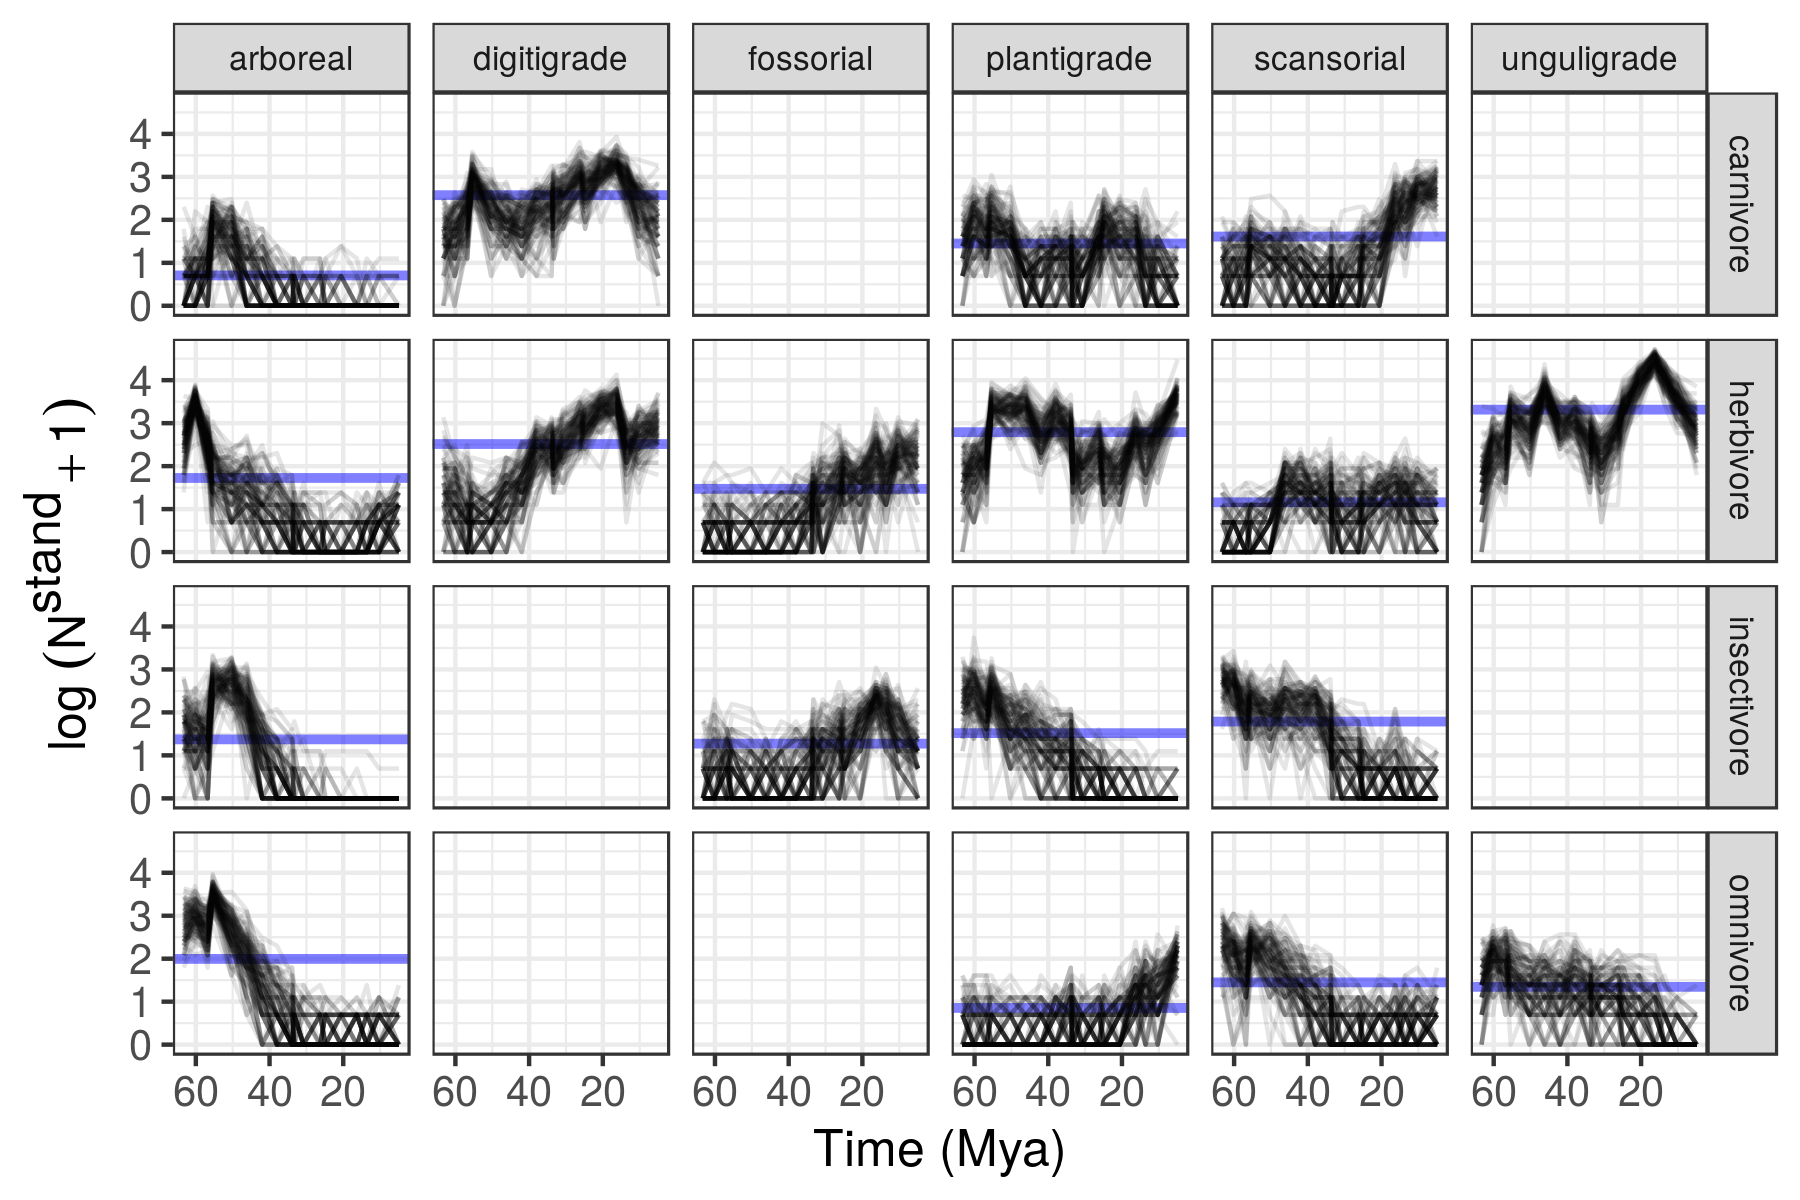
\includegraphics[width=\textwidth,height=0.8\textheight,keepaspectratio=true]{figure/ecotype_diversity}
  \caption[Estimated mammal ecotype log-diversity for the Cenozoic]{Posterior of standing log-diversity of North American mammals by ecotype for the Cenozoic as estimated from the birth-death model; 100 posterior draws are plotted to indicate the uncertainty in these estimates and what is technically plotted is log of diversity plus 1. The dramatic differences between diversity estimates at the first and second time points and the penultimate and last time points in this series are caused by well known edge effects in discrete-time birth-death models caused by \(p_{\_, t = 1}\) and \(p_{\_, t = T}\) being partially unidentifiable \citep{Royle2008}; the hierarchical modeling strategy used here helps mitigate these effects but they are still present \citep{Gelman2013d,Royle2008}.}
  \label{fig:ecotype_diversity}
\end{figure}

\end{document}


%\documentclass[12pt,letterpaper]{article}

\usepackage{amsmath, amsthm}
\usepackage{microtype, parskip}
\usepackage[comma,numbers,sort&compress]{natbib}
\usepackage{lineno}
\usepackage{docmute}
\usepackage{caption, subcaption, multirow, morefloats, rotating}
\usepackage{wrapfig}
\usepackage{attrib}

\frenchspacing

\begin{document}

\section*{Discussion}

%Over time both the stage and the actors change, but not at the same rate. As the actors change, do their parts remain?
Both the composition of a species pool and its environmental context change over time, though not necessarily at the same rate. Local communities, who's species are drawn from the regional species pool, have ``roles'' in their communities defined by their interactions with a host of biotic and abiotic interactors (i.e. species niche). For higher level ecological characterizations like ecotypes and guilds, these roles are broadly defined and not defined by specific interactions but the genre of interactions that species within that grouping participate in. The diversity of species within an ecotype or guild can be stable over millions of years despite constant species turnover \citep{Jernvall2004,Slater2015c} CITATIONS. This implies that the size and scope of the role of an ecotype or guild is preserved even as the individual interactors change. This also implies the structure of regional species pools can be constant over time despite a constantly changing set of ``players.''

Comparison of the pure-presence model to the birth-death model support the conclusion that regional species pool dynamics cannot simply be described by a single occurrence probability and is instead better modeled as the result of both origination and extinction. Additionally, changes to ecotypic composition of the North American regional species pool are driven primarily by variation in origination rates. These aspects of how regional species pool diversity is shaped is not observable from studies of the Modern CITATION.


Extinction rate for the entire regional species pool through time is highly variable and demonstrates a saw-toothed pattern around an apparently constant mean. While a constant mean extinction rate is consistent with previous observation \citep{Alroy1996a,Alroy2000g}, the degree to which extinction rate is actually variable may not have been equally appreciated. What is most consistent with previous observations \citep{Alroy1996a,Alroy2000g}, however, is that diversity seems to be most structured by origination than extinction.


Arboreal taxa disappear over the Cenozoic, with massive disappearance by the Paleogene-Neogene transition \(\sim\)22 Mya. This is consistent with one of the two possible patterns that would result in arboreal taxa having a greater extinction risk than other ecotypes: Paleogene-Neogene are different and while the earliest Cenozoic may have been neutral wrt arboreal taxa, they disappeared quickly over the Cenozoic which may account for their higher extinction risk.

Digitigrade carnivores have a relatively stable diversity history through the Cenozoic and could be characterized as varying around a constant mean diversity. The ecotypie has a large amount of overlap with the carnivore guild which has been the focus of much research CITATIONS. This result is consistent with some form of ``control'' on the ecotype, such as environmental stability, diversity-dependence, or similar \citet{Slater2015c,Silvestro2015b}.

Both digitigrade and unguligrade herbivores increase in diversity over the Cenozoic. The increase of these cursorial forms is consistent with the gradual opening up of the North American landscape CITATION. Only these herbivore from increase in diversity over the Cenozoic which may indicate a long shift in the interactors associated with those ecotypes leading to increased contribution to the regional species pool. This result may be comparable to the increasing percentage of hypsodont (high-crowned teeth) mammals in the Neogene of Europe being due to an enrichment of hyposodont taxa and not a depletion of non-hypsodont taxa.



What these results support is a gradual change to the ecotypic diversity of the regional species pool for the Cenozoic. The rapidity of Cenozoic environmental change is worth discussing. If change is rapid, ecotypic composition of species pool does not seem to track environmental change. If change is gradual then there is the possibility that changes to ecotypic composition may be tracking environmental change.

If plant phase is associated with differences in ecotype occurrence this is interpreted to mean that ecotype enrichment or depletion is due to to associations between that ecotype and whatever plants are dominate at that time.

Temperature affects very few of the occurrence, origination, or survival probabilities of the mammal ecotypes except for a negative relationship between temperature and the origination probabilities of digitigrade carnivores, and both digitigrade and unguligrade herbivores. The origination probabilities and diversity of these three groups all increase over the Cenozoic as average global temperature decreased. This result coupled with the lack of relationship between temperature and the other ecotypes may be responsible for the continued confusion surrounding the impact of temperature on mammal diversity and diversification \citep{Alroy1996a,Alroy2000g,Figueirido2012,Janis1993c,Blois2009}.

What is the comparative size of the effects of plant phase and temperature? Both seem of ``equal'' importance in the sense that they have similar effect sizes on the ecotypes. Perhaps focusing on temperature and not considering other measures of environmental context has been a mistake and perhaps led to increasing confusion in discussions of how ``environment'' effects mammal diversity and diversification. The environment or climate is not just global or regional temperature, it is the set of all possible biotic and abiotic interactions. By including more descriptors of species' environmental context a more complete ``picture'' of the diversification process is inferred.


The effect of species mass on either occurrence or origination and extinction was not allowed to vary by ecotype or environmental context even though it is not known if this is the case or not CITATION. The primary reason for this modeling choice was that this study focuses on ecotypic based differences in either occurrence, or origination and extinction. Allowing the effect of body size to vary by ecotype, time, and environmental factors would increase the overall complexity of the model, something that I felt was not necessary because the overall scope of the study. Instead, body size was included in order to control for its possible underlying effects CITATION. A control means that if there is variation due to body mass, having a term to ``absorb'' that effect is better than ignoring it which may affect other parameter estimates. Additionally, the effect of body size was allowed to have a second-order polynomial form and no higher order polynomials were considered; this was done because it is hard to conceive of a more complex third- or higher-order relationship between body size and the other parameters. Additionally, nonlinearity is rarely if ever considered in the first place, so the simple act of estimating a potential second-order relationship is an opportunity to test more complex hypotheses of the effects of body size on macroevolutionary and macroecological processes.

The only covariate allowed to affect sampling probability was mass and only as a linear predictor. Other covariates, such as the environmental factors considered here, could have affected the underlying preservation process that limits sampling probability. Their exclusion as covariates of sampling/observation was the product of a few key decisions: model complexity, model interpretability, the scope of this study, and a lack of good hypotheses related to these covariates to warrant their inclusion. It should be noted that in other similar studies that use a hidden birth-death model to handle simultaneous estimation of sampling, origination, and extinction have not considered the possible effects of covariates, both species traits and environmental factors, on sampling CITATION.

The time scale available with paleontological data is much greater than that obtainable from modern ecological studies, even long running observations CITATION. Specifically, the temporal scale of paleontological data allows for the complete turnover of a species pool to be observed, something that is impossible in ``real time.'' However, paleontological data is very limited in its spatial resolution, so the analysis of how the ecotypic diversity local communities change over time and how that is also the product of larger scale regional turnover remains unanswered.

The potential effects of common ancestry (i.e. phylogeny) on origination and extinction are not directly considered in this analysis. While a birth-death process approximates the speciation-extinction process underlying the phylogeny \citep{Silvestro2014a} this is not same as considering how the similarity between closely related species may affect the estimates of the effects of species traits to environmental factors on both origination and extinction \citep{Smits2015b,Harnik2014}. One of the principle barriers to the inclusion of the effect of phylogeny in either the pure-presence or birth-death models is computational; with well over 1000 tips, the calculation of the scale parameter defining the phylogenetic effect would be very slow and further increase the already slow computation time necessary for both the marginalization of the discrete occurrence histories and data augmentation already included in both models.

Phylogenetic comparative community ecology and phylogenetic comparative biogeography also discusses how the macroevolutionary processes helps structure an observed community, though it is not necessarily phrased that way. However, that community did not form in isolation but it the result of many factors interacting over time including incumbency, competition, limiting similarity, etc.







\end{document}



\section*{Acknowledgements}
I would like to thank K. Angielzcyk, M. Foote, P. D. Polly, and R. Ree for helpful discussion and advice. This entire study would would not have been possible without the Herculean effort of the many contributors to the Paleobiology Database. In particular, I would like to thank J. Alroy and M. Uhen for curating most of the mammal occurrences recorded in the PBDB. This is Paleobiology Database publication XXX.


%\bibliographystyle{amnatnat}
%\bibliography{newbib,packages}


\end{document}
